\label{chap.4}
This chapter reports the experiments in the order the work was done. Every number comes from a results file in the
repository (Appendix~A); release v2 numbers use the corrected labels.

\section{Experimental Setup}

\begin{itemize}
  \item \textbf{Training:} Kaggle notebooks, NVIDIA T4 GPU (16\,GiB). Each staging run took about 20 minutes; the v2
  report model's LoRA training took 169 minutes.
  \item \textbf{Inference and evaluation:} a Windows x86 PC (CPU only, about 7\,GB free RAM); llama.cpp b10927;
  Python 3 with PyTorch, MNE and SciPy.
  \item \textbf{Edge simulation (L1):} a second Windows PC with Docker Desktop; a Linux x86-64 container (Python
  3.12, CPU-only PyTorch, llama.cpp b10927 built from source) limited to 4 CPUs and 16\,GiB, started with
  \texttt{--network none} and the project mounted read-only.
  \item \textbf{Determinism:} report generation at temperature 0, seed 0, fixed grammar and pinned chat template.
  \item \textbf{Edge target (not yet measured):} Raspberry Pi 5, 4$\times$ Cortex-A76 at 2.4\,GHz, 16\,GB LPDDR4X, NVMe.
\end{itemize}

\section{Datasets:}

Sleep-EDFx as described in Section~\ref{sec:dataset}, with these evaluation configurations:
\begin{itemize}
  \item \textbf{Held-out test:} 15 subjects, 29 nights, 33,365 epochs; locked, one logged read per model.
  \item \textbf{Standard benchmark (B1):} Sleep-EDF-78 (SC only, 78 subjects, 153 nights), 10-fold subject-wise
  cross-validation, trained from scratch (no warm start, no distillation); 78/78 subjects and 153/153 recordings
  each appear in exactly one fold.
  \item \textbf{Cohort transfer:} train on 62 SC subjects, test on all 22 ST subjects.
  \item \textbf{Path B (raw EDF):} the 31 dev nights cropped at lights-off to a 12-hour device-like window, with no
  expert hypnogram; the study period is estimated by the model.
  \item \textbf{Report model:} 123 training and 14 validation nights with reference targets; 31 dev nights for
  selection; the 29 test nights once (pre-registered).
\end{itemize}

\section{Evaluation Metrics:}

\begin{itemize}
  \item \textbf{Staging:} accuracy; \textbf{Cohen's $\kappa$} (primary, robust to class imbalance); macro-F1 and
  per-class F1; bootstrap 95\% CIs resampled \emph{by subject}; paired Wilcoxon signed-rank tests per subject.
  \item \textbf{Calibration:} expected calibration error (ECE, 15 bins); night-level Pearson / Spearman correlation
  between mean entropy and $\kappa$.
  \item \textbf{Reports:} verified (no violation); \textbf{5/5} (verified and all mandatory items covered);
  violations; \textbf{numeric fidelity} (cited values equal to packet values); flawed reports released; two-sided
  95\% Clopper--Pearson lower bound (for $n/n$ successes, $0.025^{1/n}$).
  \item \textbf{Agent:} outcome and reason codes per scenario; invariants I1--I8; byte-identical reruns; wall time.
  \item \textbf{Edge:} network reachability, secret scan, cross-platform staging parity (max $|\Delta p|$, identical
  hypnograms), wall time and peak memory per night; tokens/s (analytical for the Pi).
\end{itemize}

\section{Experimental Design}

\textbf{Baseline methods:} the inherited 649,229-parameter model (re-evaluated honestly); retrained teachers E0,
E1a, E1b; a non-distilled student of the same size (the control for every KD experiment); the v1 student N4kd;
YASA 0.8.1; the published models of Table~\ref{tab:published}; and, for reports, five untrained small models and
the untrained Llama-3.2-3B.

\subsection{Experimental Scenarios:}

\begin{enumerate}
  \item \textbf{Exposure gradient:} the inherited model on epochs it trained on, on the same subject's other night,
  and on an unseen subject.
  \item \textbf{KD vs control:} students distilled from teachers of different quality against an identical student
  trained on hard labels only.
  \item \textbf{Encoder and channel ablations:} receptive field, raw EEG zeroed, EOG added.
  \item \textbf{Architecture ablation (5-fold CV, same labels):} \texttt{base} $\rightarrow$ \texttt{full\_eeg} (TF +
  local context + recipe) $\rightarrow$ \texttt{full} (+ EOG).
  \item \textbf{Missing channel:} v2 evaluated with the EOG input removed.
  \item \textbf{Report-model selection:} reference run, grammar ablation, LoRA students on dev, one test run.
  \item \textbf{Verifier ablation:} gate on / gate off / gate and grammar off, on 31 dev nights, for v1, v2 and the
  untrained model.
  \item \textbf{Agent fault scenarios:} 15 scenarios on real EDF files and injected report-model faults.
  \item \textbf{Sampling rates and line noise:} 128 and 256\,Hz recordings; 49/50\,Hz noise injected at 0.25--2$\times$
  EEG RMS.
  \item \textbf{Reproducibility:} Path B twice per dev night in fresh runtime directories with the real model.
  \item \textbf{Edge containers:} environment checks; staging on all 31 dev recordings; the report model on all 31
  dev packets; three raw nights end to end; and staging on 8 nights under ARM64 emulation --- all inside offline,
  resource-limited containers and compared with the reference PC.
\end{enumerate}

\subsection{Parameter Tuning:}

\begin{itemize}
  \item Distillation: $\alpha = 0.5$, $T = 3$, fixed for every reported run.
  \item Staging: AdamW, lr $3\times10^{-4}$, 75 epochs, model selection on \textbf{validation} macro-F1; 3 seeds for v2.
  \item Calibration temperature, decoder, night-confidence tiers and the N1 flag threshold: fitted on validation
  only, applied unchanged to test.
  \item Report model: hyperparameters pre-registered and locked before training (Table~\ref{tab:sft}).
  \item Agent thresholds (quality, study period, resources): set in the policy file and calibrated on train/dev.
\end{itemize}

\begin{table}[htbp]
\centering\small
\caption{Report-model training configuration (identical for v1 and v2).}
\label{tab:sft}
\begin{tabularx}{\textwidth}{lY}
\toprule
Parameter & Value \\
\midrule
Base models & Llama-3.2-3B-Instruct; Qwen2.5-1.5B-Instruct \\
Method & LoRA (PEFT), rank 16, $\alpha$ 32, dropout 0.05, on q/k/v/o and MLP projections \\
Optimiser & lr $2\times10^{-4}$, cosine; effective batch 8; 3 epochs; seed 0 \\
Data & 123 training nights, 14 validation nights; targets = reference claim sets that pass the verifier, serialised in the grammar's field order \\
Max sequence & 3,072 tokens \\
Export & F16 $\rightarrow$ Q4\_K\_M with llama.cpp b10927 \\
\bottomrule
\end{tabularx}
\end{table}

\section{Results}

\subsection{Stage 1 --- Knowledge distillation (v1, stored labels, historical)}\label{sec:res-kd}

\textbf{The inherited model had memorised people} (Table~\ref{tab:exposure}, Figure~\ref{fig:exposure}). Its
reported $\kappa$ of 0.6663 is reproduced to within 0.0008 as a blend of the leaked and clean measurements,
confirming leakage as the explanation.

\begin{table}[htbp]
\centering\small
\caption{Exposure gradient of the inherited model.}
\label{tab:exposure}
\begin{tabular}{lrrrr}
\toprule
Exposure level & $\kappa$ & Macro-F1 & N3 F1 & REM F1 \\
\midrule
Same recording (trained on) & 0.8058 & 0.8036 & 0.889 & 0.876 \\
Same subject, other night (leaked) & 0.6797 & 0.7173 & 0.837 & 0.718 \\
\textbf{Unseen subject} & \textbf{0.5066} & \textbf{0.4107} & \textbf{0.000} & \textbf{0.184} \\
\bottomrule
\end{tabular}
\end{table}

\begin{figure}[htbp]
\centering
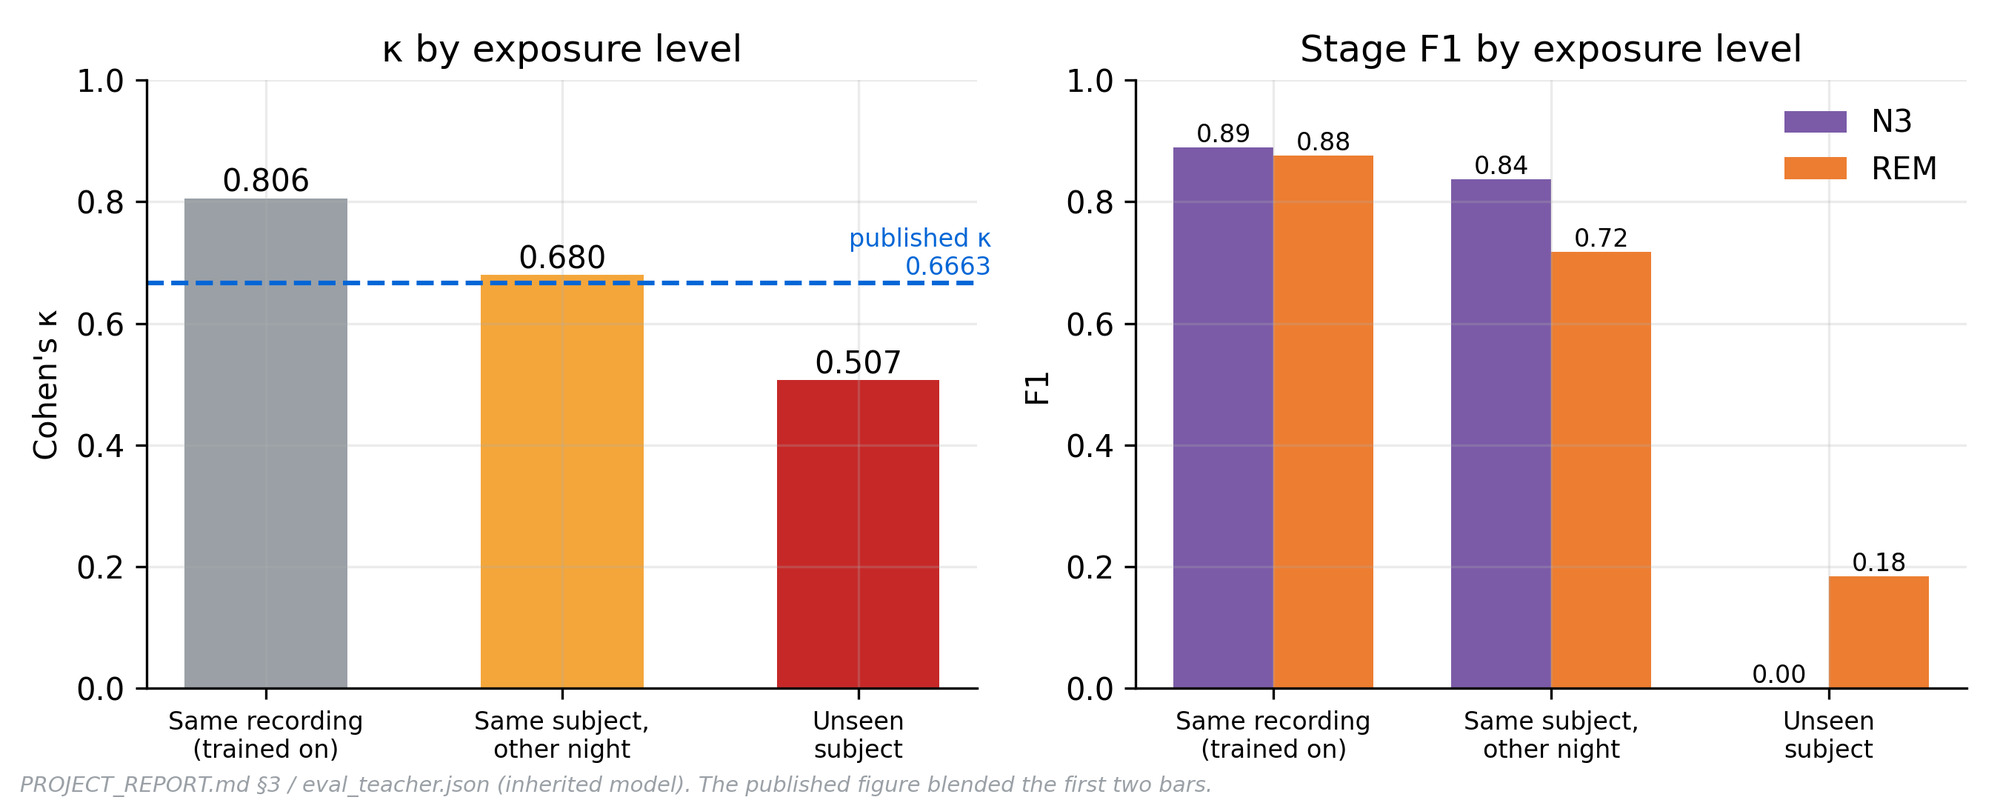
\includegraphics[width=0.8\textwidth]{F3_exposure_gradient.jpg}
\caption{Exposure gradient: what the inherited model had memorised.}
\label{fig:exposure}
\end{figure}

\begin{table}[htbp]
\centering\small
\caption{Distillation experiments, held-out test (15 subjects), stored labels (v1 era).}
\label{tab:kd}
\begin{tabular}{lrrr}
\toprule
Model & Params & $\kappa$ & Macro-F1 \\
\midrule
E0 teacher (faithful retrain) & 649,229 & 0.5122 & 0.6063 \\
E1b teacher (double class-weighting fixed) & 649,229 & 0.6055 & 0.6548 \\
Student distilled from E0 & 121,099 & 0.5925 & 0.6611 \\
Student distilled from E1b & 121,099 & 0.6134 & 0.6708 \\
\textbf{Student, no distillation (control)} & 121,099 & \textbf{0.6449} & \textbf{0.6915} \\
Student, multi-scale encoder & 139,606 & 0.6992 & 0.7407 \\
Ensemble teacher (3 students) & 412,311 & 0.7140 & 0.7542 \\
Student distilled from the ensemble (v1, N4kd) & 139,606 & 0.7001 & 0.7376 \\
\bottomrule
\end{tabular}
\end{table}

\textbf{Findings} (Table~\ref{tab:kd}):
\begin{enumerate}
  \item \textbf{Fixing the teacher's loss mattered more than capacity.} E1a's focal loss applied class weights twice,
  suppressing N2; fixing it (E1b) raised test $\kappa$ from 0.559 to 0.606 with no added parameters
  (Figure~\ref{fig:ladder}).
  \item \textbf{Naive KD hurt.} Both distilled students scored below the control, significantly. The student had
  outgrown its teacher during training, so half of every gradient pulled a good model towards a worse one
  (Figures~\ref{fig:kdmech} and~\ref{fig:penalty}). \emph{A teacher must exceed the student's own undistilled
  performance before its soft targets carry usable information}; no choice of $\alpha$ or $T$ can fix this.
  \item \textbf{The encoder could not see sleep.} Its receptive field was 0.25\,s, too short for any sleep
  microstructure. Widening it to 8.75\,s moved the raw EEG from contributing nothing to driving 71\% of predictions
  and raised N1 F1 by 0.092.
  \item \textbf{An ensemble of comparable, diverse students is a teacher that works.} It exceeds each member, and
  distilling it removed the penalty. On accuracy the distilled student tied its hard-label twin; what improved was
  \textbf{calibration}: ECE fell by about a third and REM-latency error nearly halved (Figure~\ref{fig:calib}).
  \item \textbf{The evaluation became the limit.} 5-fold subject-level CV showed the original validation split was
  an unrepresentative draw ($\kappa$ 0.7143 across folds vs 0.6763 on that split; fold SD 0.0193), larger than the
  whole distillation effect on $\kappa$ (0.0008).
\end{enumerate}

\begin{figure}[htbp]
\centering
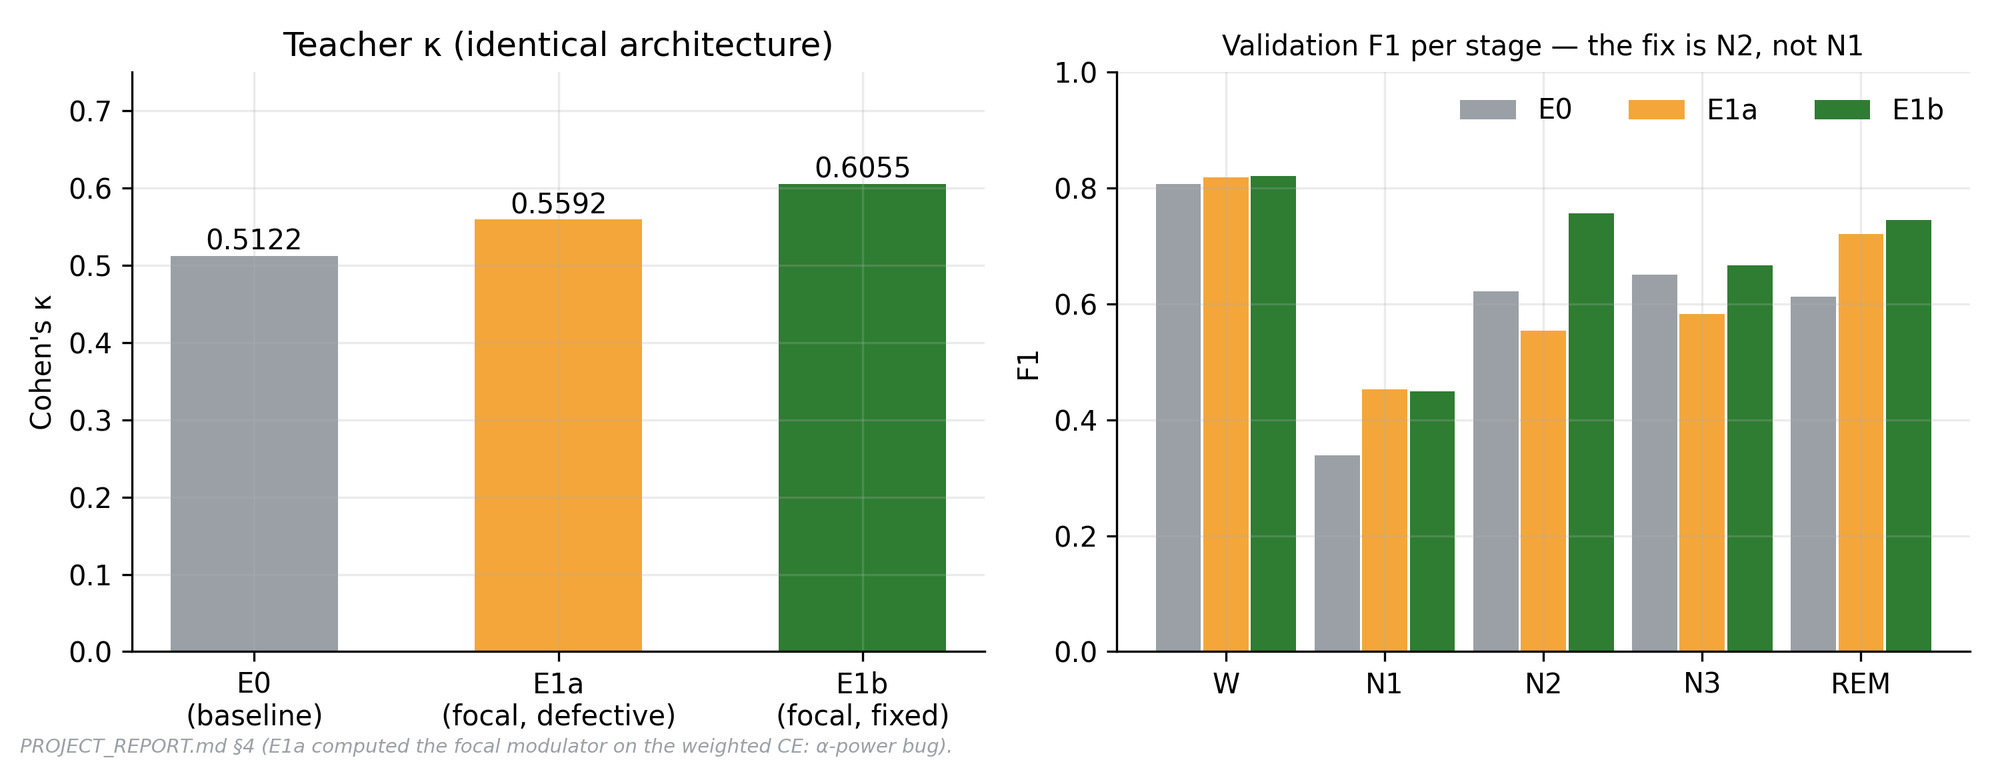
\includegraphics[width=0.75\textwidth]{v1_F6_teacher_ladder.jpg}
\caption{Teacher ladder E0 $\rightarrow$ E1a $\rightarrow$ E1b (v1 era, stored labels).}
\label{fig:ladder}
\end{figure}

\begin{figure}[htbp]
\centering
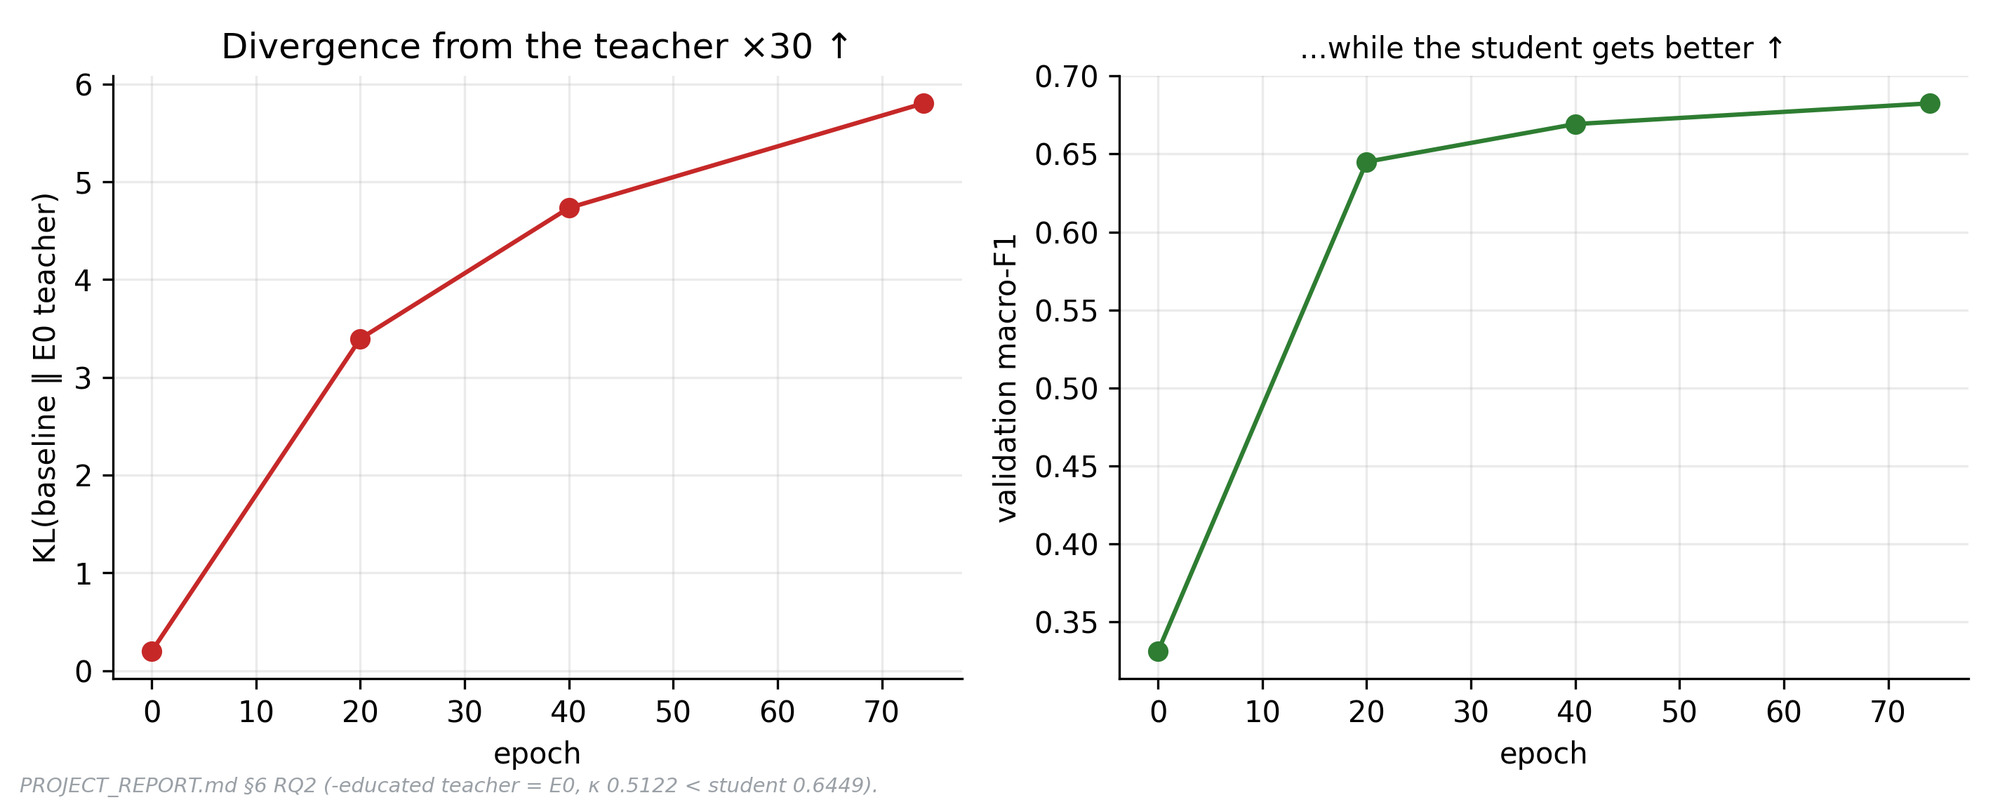
\includegraphics[width=0.85\textwidth]{v1_F11_kd_mechanism.jpg}
\caption{Why single-teacher distillation failed: the distillation mechanism.}
\label{fig:kdmech}
\end{figure}

\begin{figure}[htbp]
\centering
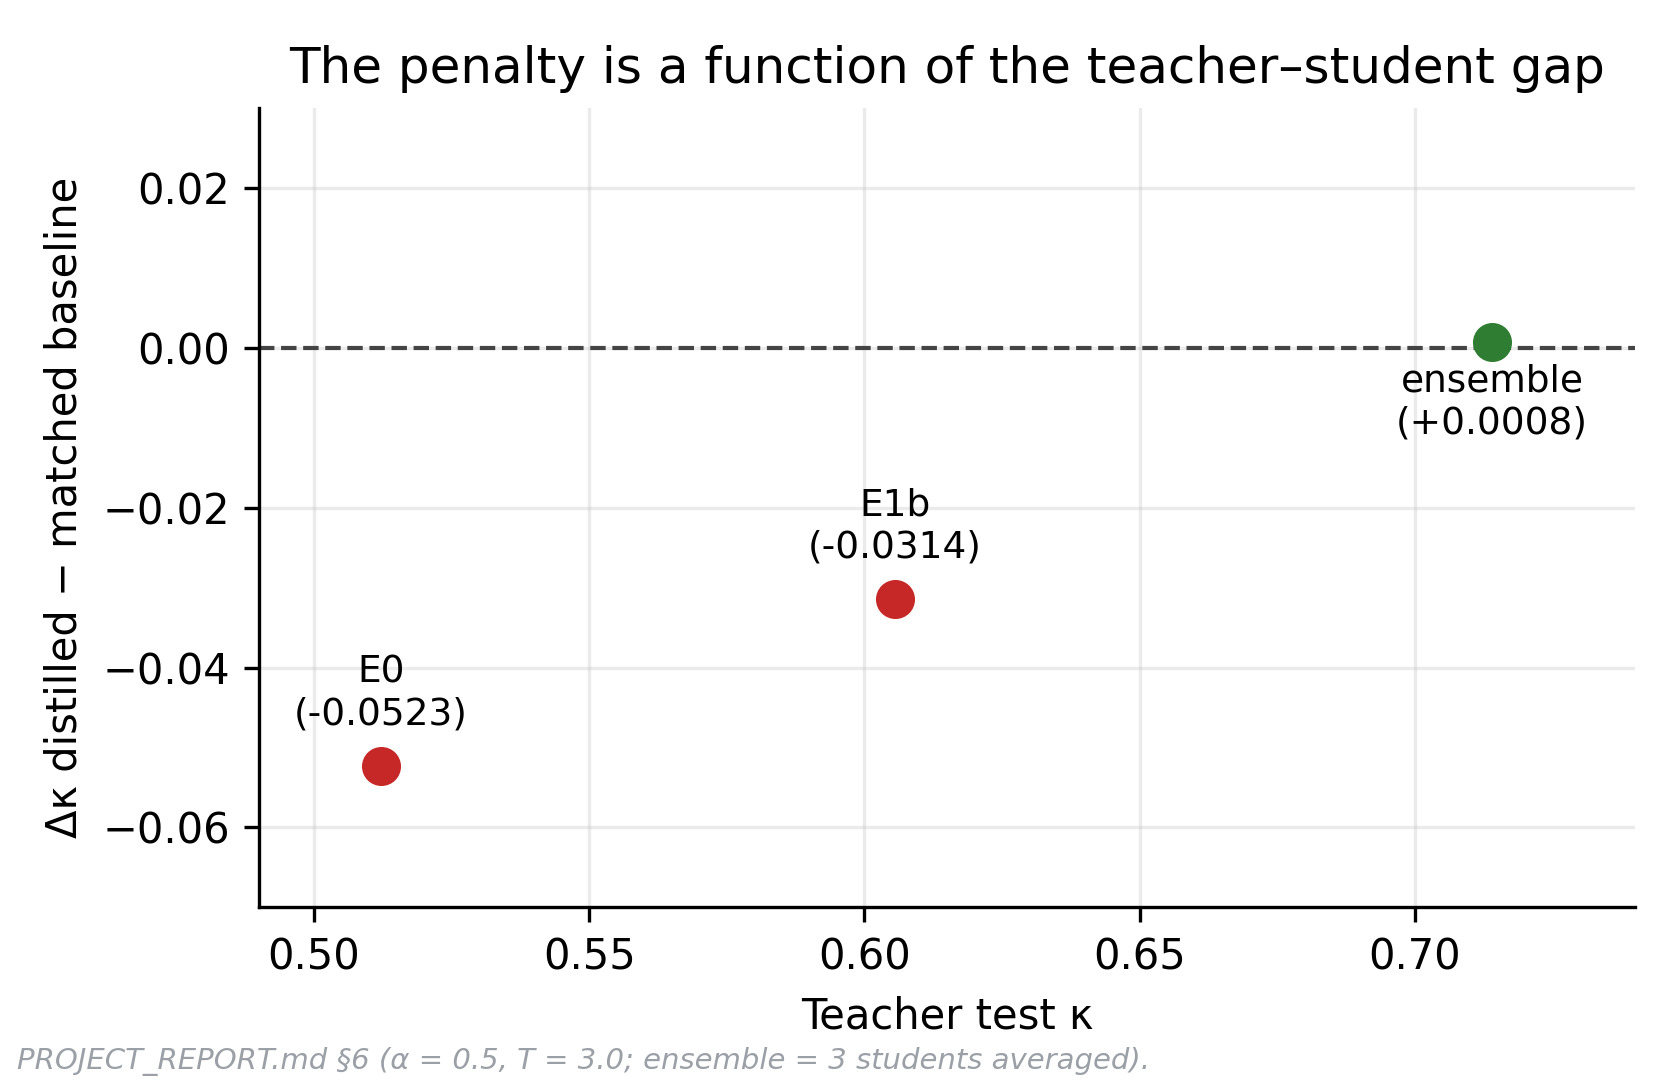
\includegraphics[width=0.7\textwidth]{v1_F12_penalty_vs_teacher.jpg}
\caption{Distillation penalty against teacher quality.}
\label{fig:penalty}
\end{figure}

\begin{figure}[htbp]
\centering
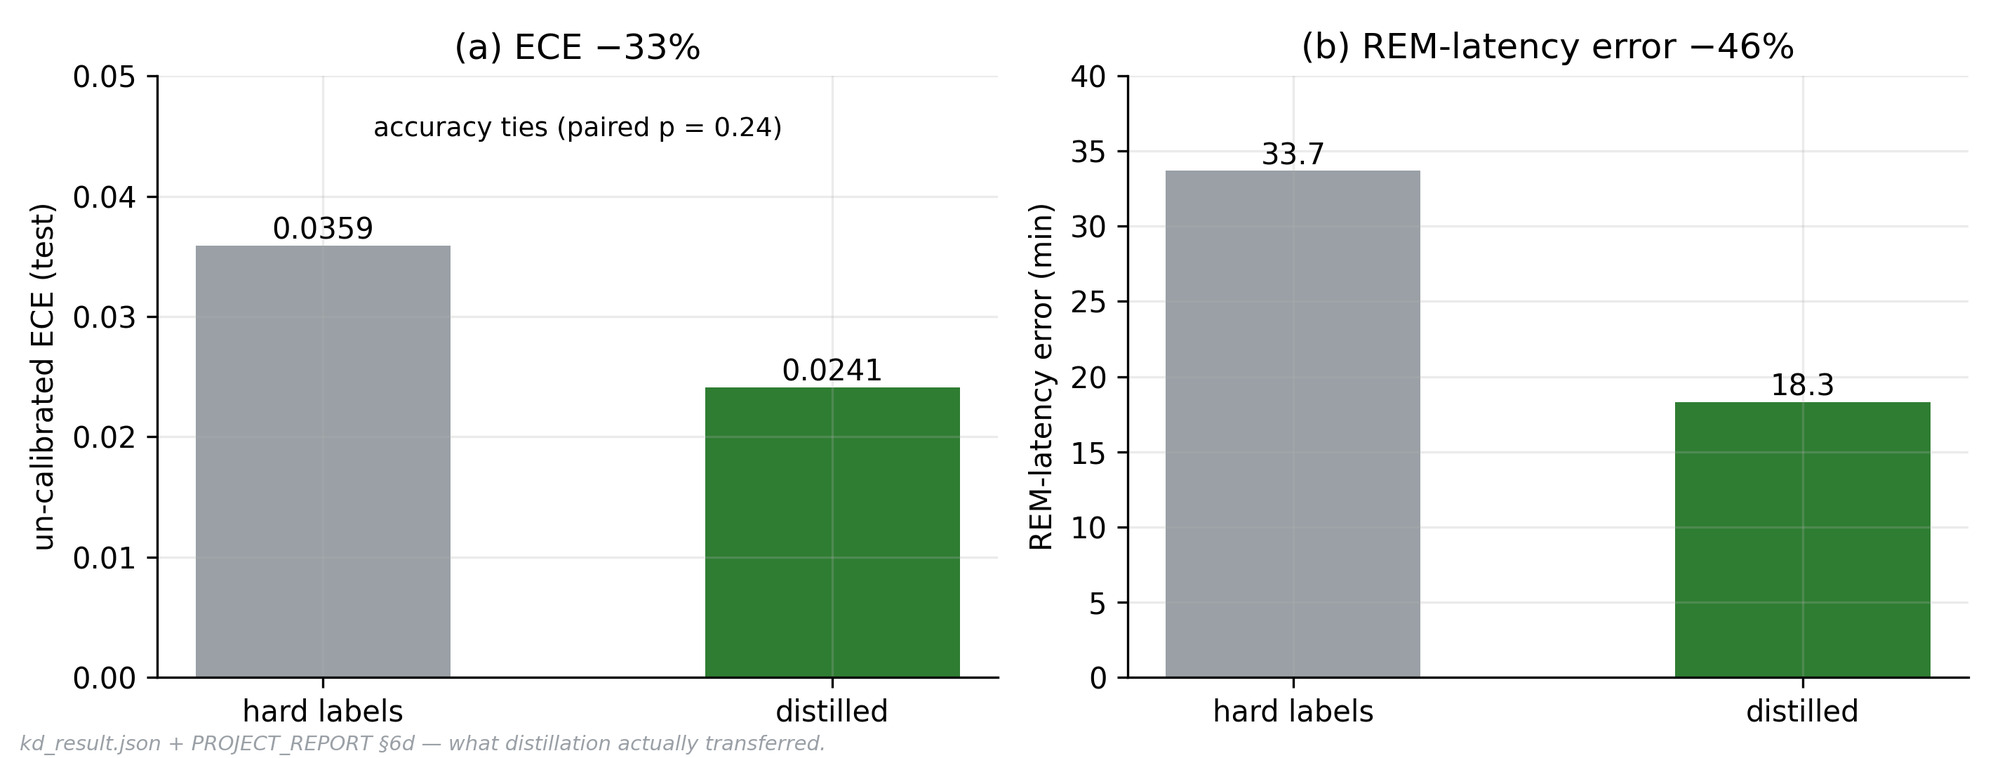
\includegraphics[width=0.85\textwidth]{v1_F13_calibration_transfer.jpg}
\caption{Calibration transfer through distillation.}
\label{fig:calib}
\end{figure}

\subsection{Stage 2 --- Student model (release v2, corrected labels)}

\begin{table}[htbp]
\centering\small
\caption{Held-out test, 15 subjects, 29 nights, 33,365 epochs, corrected labels.}
\label{tab:v2test}
\begin{tabular}{lrlrrrrr}
\toprule
Model & Params & Input & Acc. & $\kappa$ & MF1 & N1 F1 & REM F1 \\
\midrule
ENSmc teacher & 412,311 & EEG & 80.02\% & 0.732 & 76.91 & 48.7 & 81.8 \\
v1 student (N4kd) & 139,606 & EEG & 79.00\% & 0.718 & 75.23 & 45.5 & 78.2 \\
\textbf{v2 student (N6adv)} & \textbf{175,599} & \textbf{EEG + EOG} & \textbf{81.96\%} & \textbf{0.756} & \textbf{78.20} & \textbf{50.7} & \textbf{83.7} \\
v2, EOG removed & 175,599 & EEG & 81.10\% & 0.744 & 77.20 & 48.7 & -- \\
\bottomrule
\end{tabular}
\end{table}

\begin{itemize}
  \item v2 vs v1 (Table~\ref{tab:v2test}): $\Delta\kappa$ +0.038, 95\% CI [+0.019, +0.057]; better on 13/15
  subjects (Wilcoxon $p = 0.0009$); every stage improves (W +0.7, N1 +5.3, N2 +2.4, N3 +1.0, REM +5.3 F1 points).
  Accuracy passes 80\% on both cohorts (SC 82.1\%, ST 81.4\%).
  \item v2 beats its teacher on every metric with 43\% of its parameters. This test comparison combines label
  correction, EOG and the training recipe; the like-for-like attribution is the ablation in Table~\ref{tab:ablation}.
\end{itemize}

\begin{table}[htbp]
\centering\small
\caption{Architecture ablation, 5-fold CV, corrected labels for every arm.}
\label{tab:ablation}
\begin{tabular}{lrrl}
\toprule
Arm & Params & $\kappa$ & $\Delta\kappa$ vs base, 95\% CI \\
\midrule
\texttt{base} (v1 architecture) & 139,606 & 0.7584 & -- \\
\texttt{full\_eeg} (+ TF branch, local context, recipe) & 160,511 & 0.7653 & +0.0069 [+0.003, +0.011] \\
\textbf{\texttt{full} (+ EOG) = v2} & \textbf{175,599} & \textbf{0.7763} & \textbf{+0.0179 [+0.0095, +0.026]}, 5/5 folds \\
\bottomrule
\end{tabular}
\end{table}

\begin{figure}[htbp]
\centering
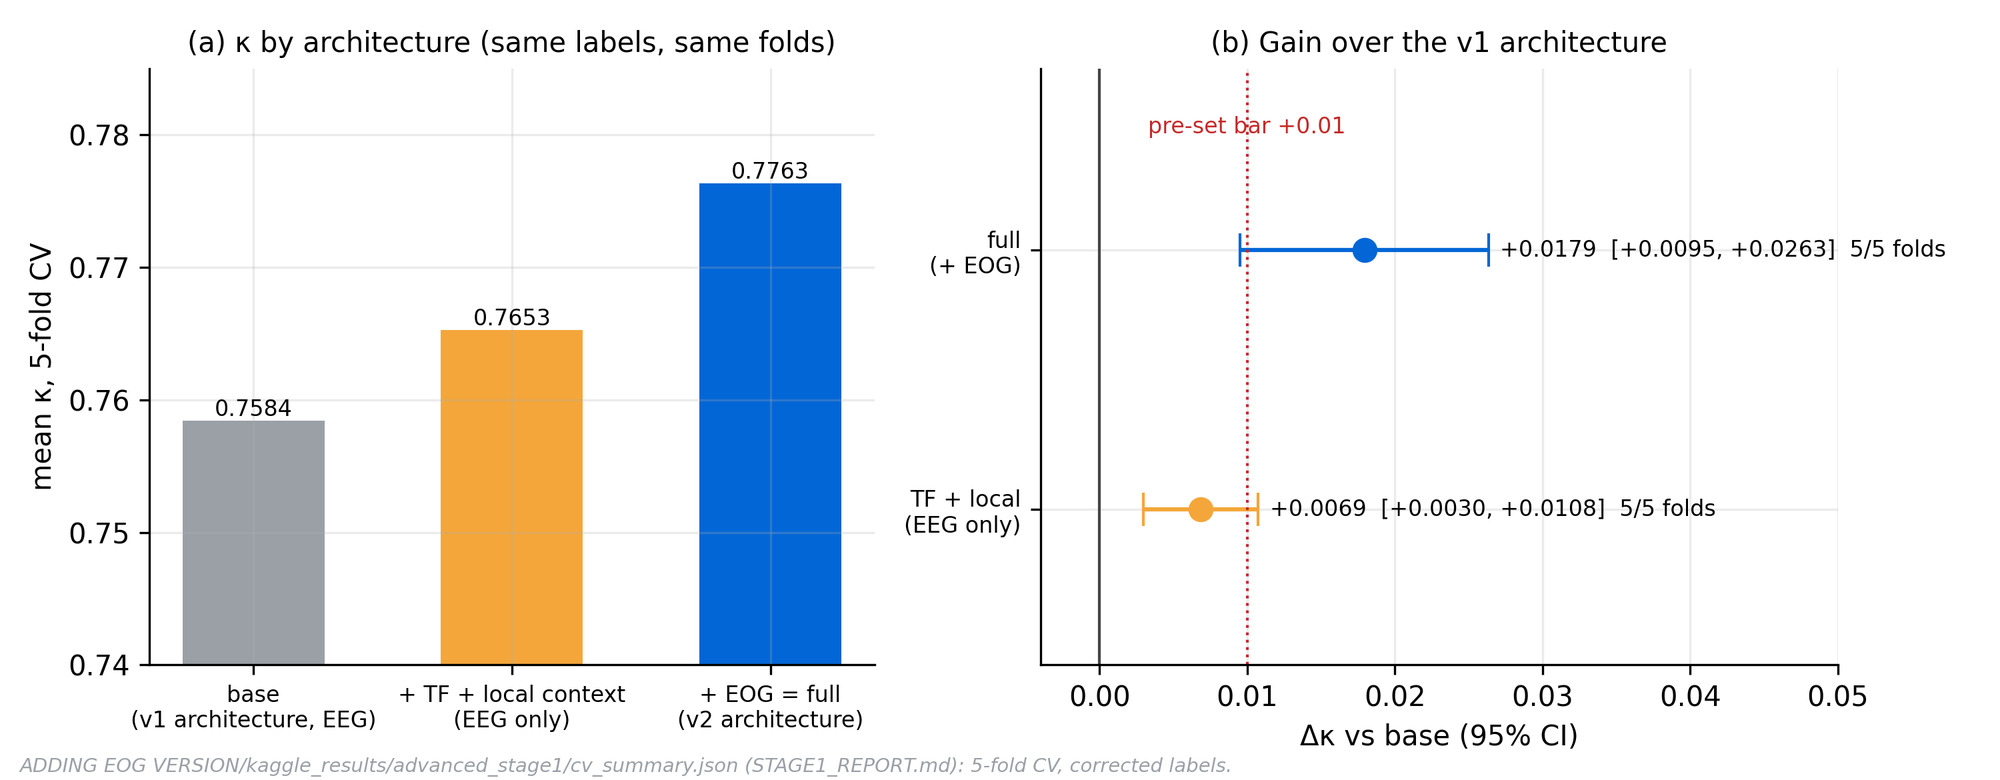
\includegraphics[width=0.85\textwidth]{F26_architecture_ablation.jpg}
\caption{Architecture ablation: what the time-frequency branch, local context and EOG add, like for like.}
\label{fig:ablation}
\end{figure}

\begin{figure}[htbp]
\centering
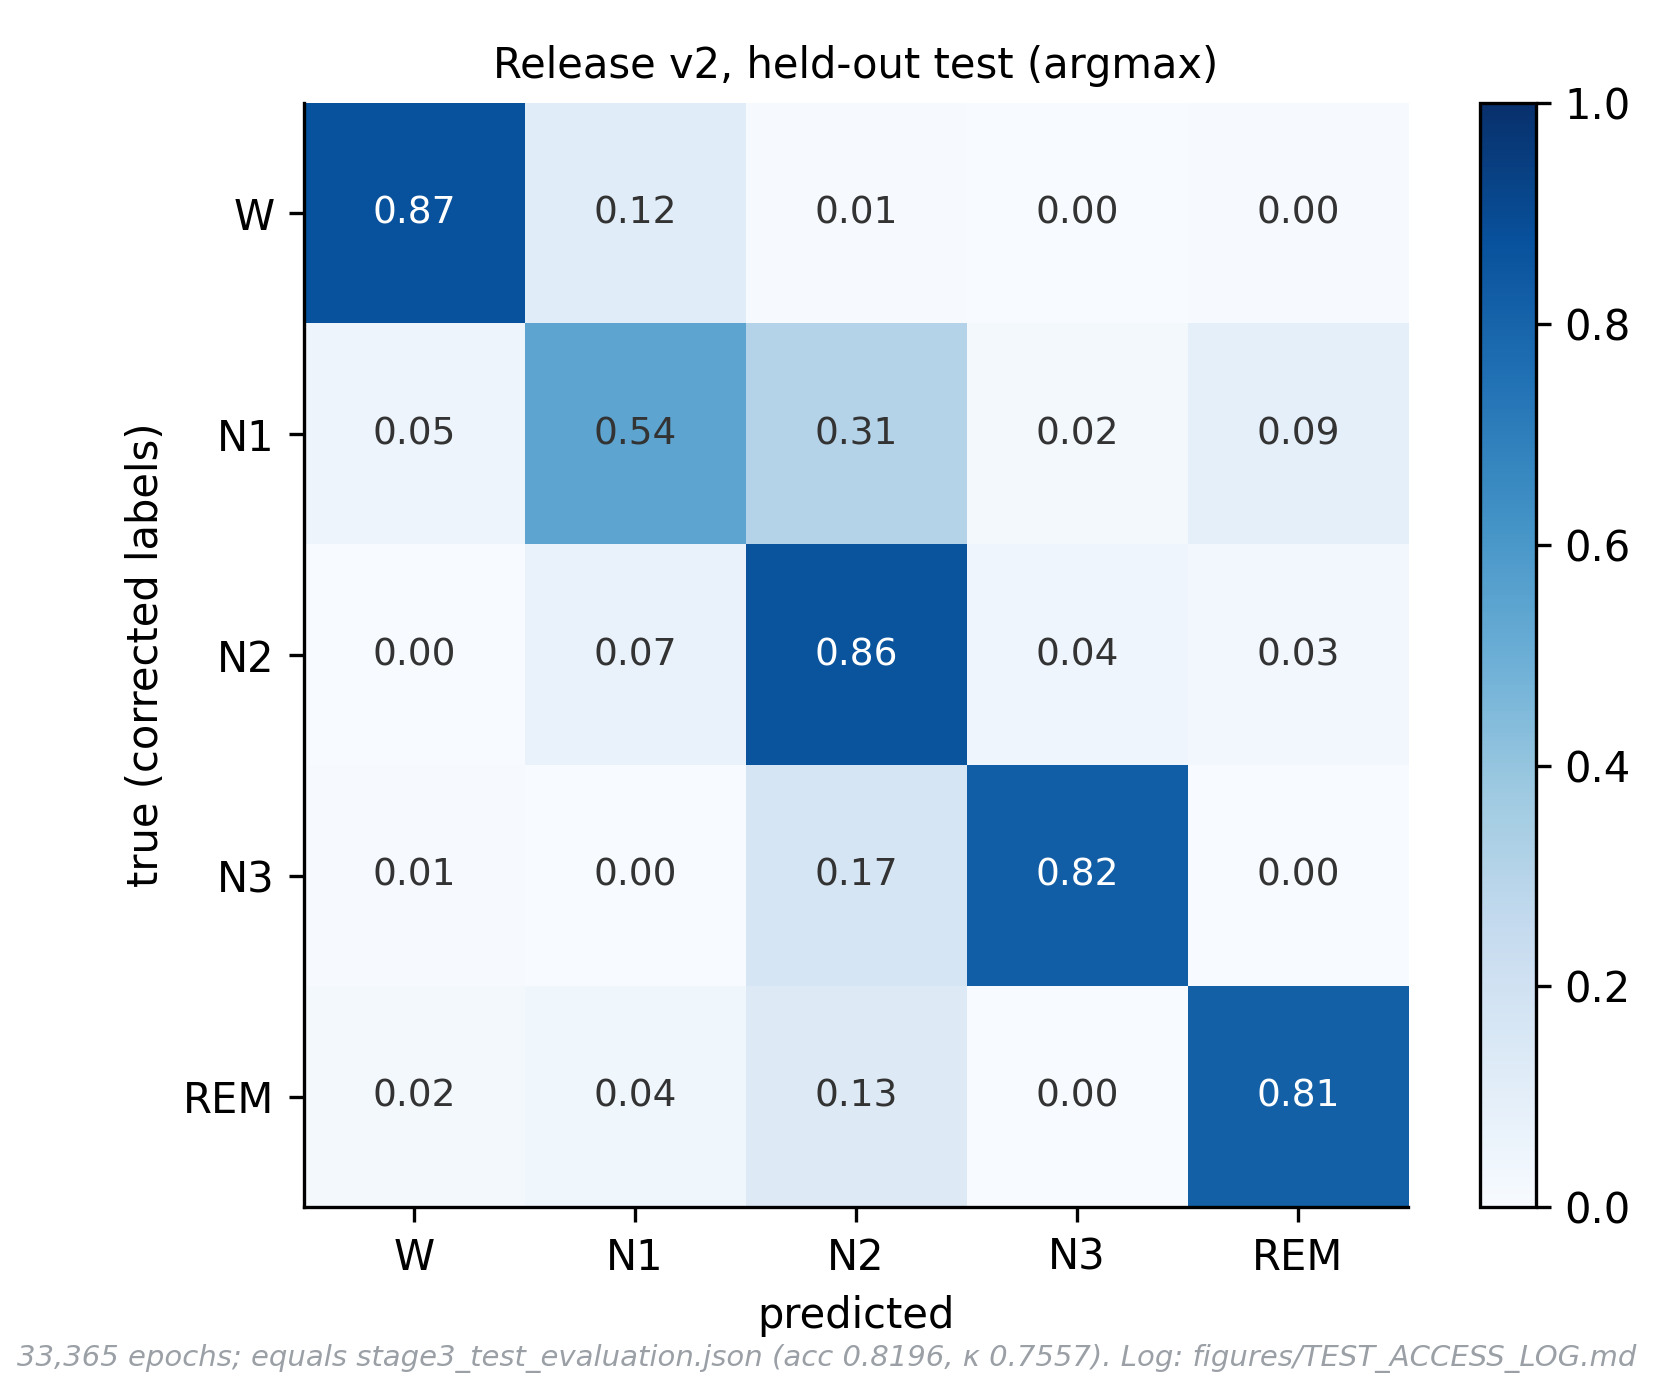
\includegraphics[width=0.75\textwidth]{F15_confusion_matrix.jpg}
\caption{Confusion matrix of release v2 on the held-out test set (corrected labels).}
\label{fig:cm}
\end{figure}

\begin{figure}[htbp]
\centering
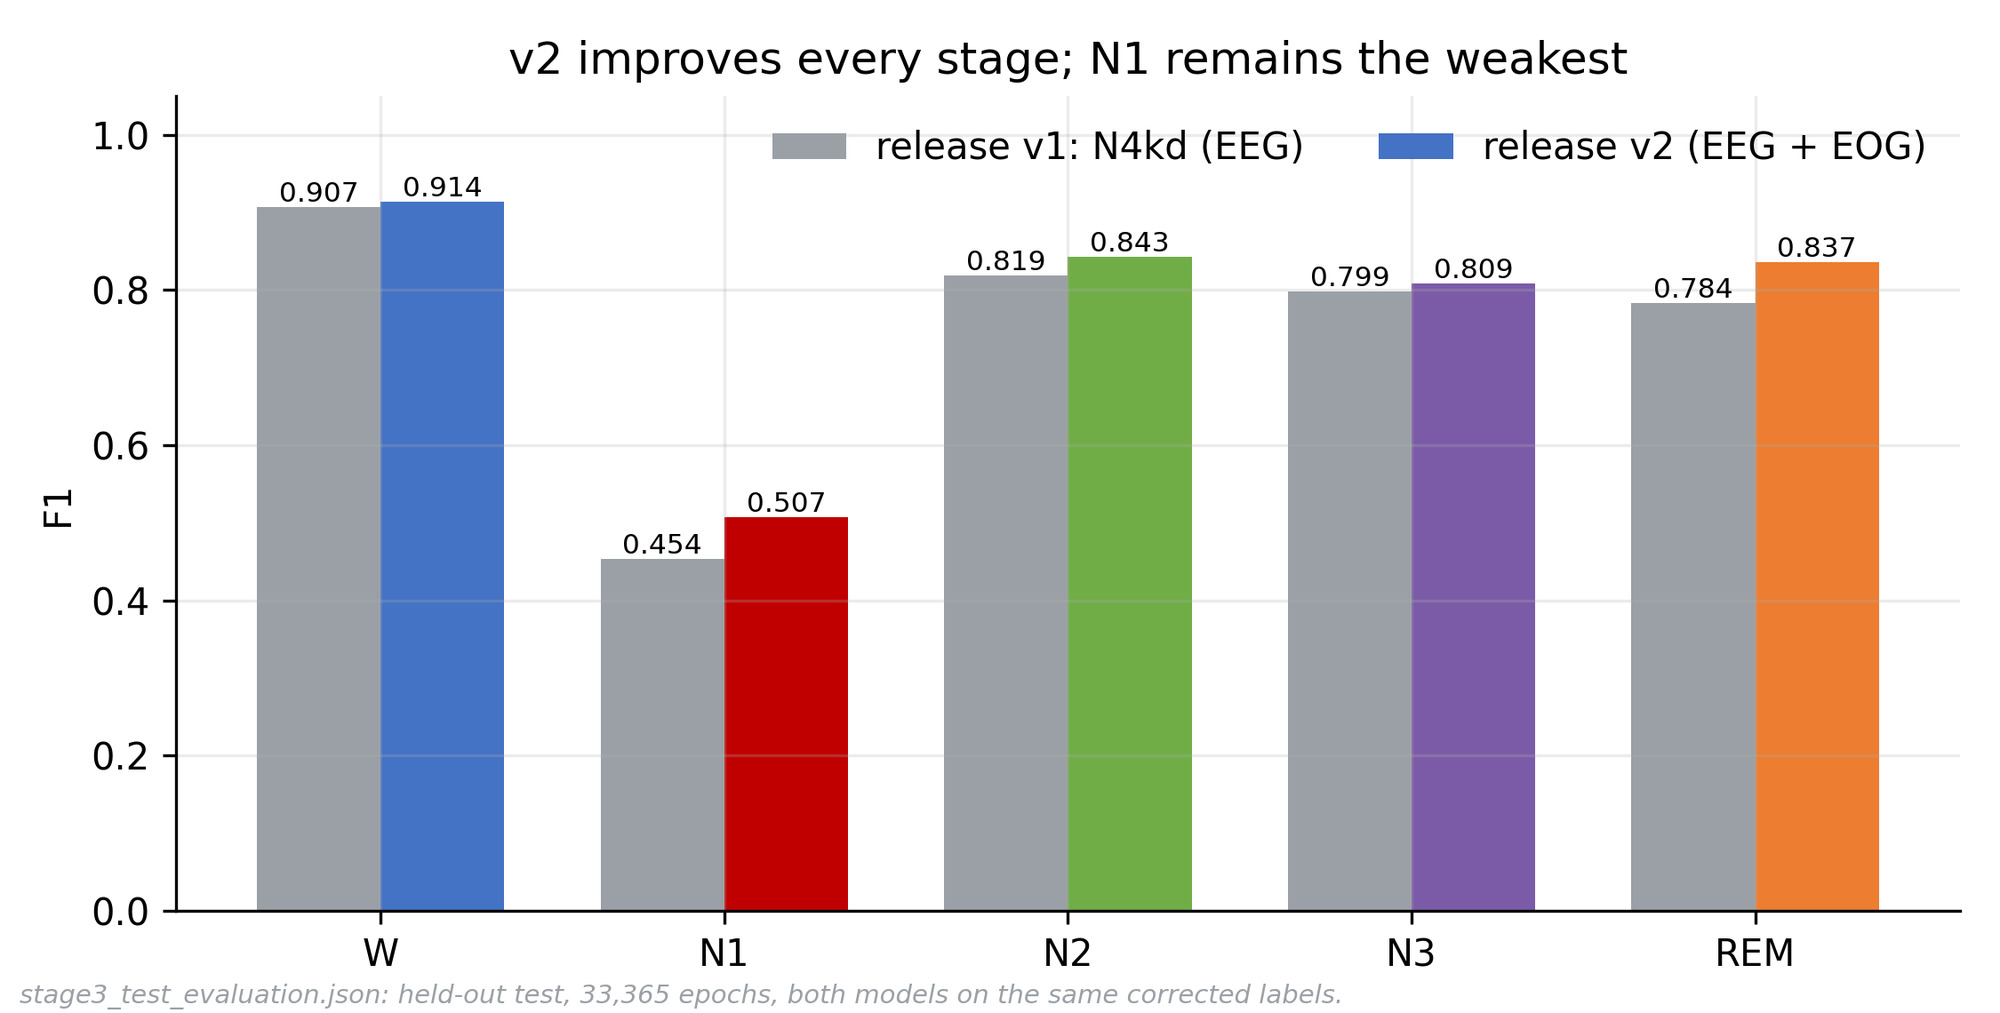
\includegraphics[width=0.85\textwidth]{F16_per_class_f1.jpg}
\caption{Per-class F1, v2 against v1 on the same labels: v2 is better on all five stages.}
\label{fig:perclass}
\end{figure}

\begin{figure}[htbp]
\centering
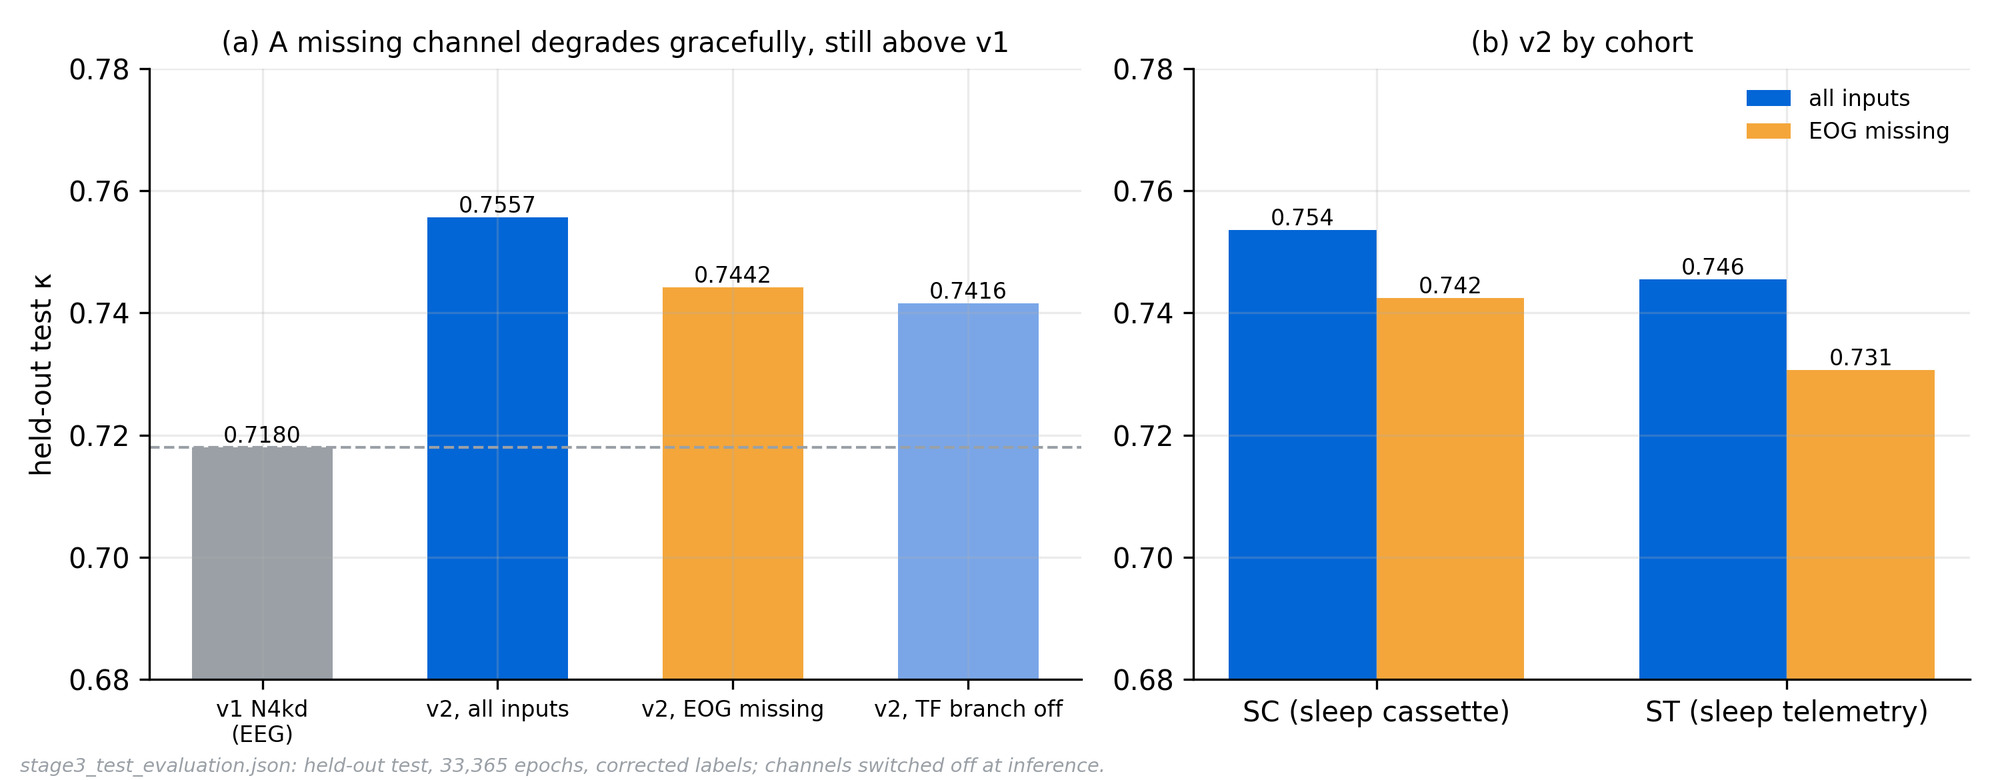
\includegraphics[width=0.85\textwidth]{F27_missing_channel_robustness.jpg}
\caption{Robustness to a missing EOG channel: 0.756 $\rightarrow$ 0.744, still above v1 (0.718).}
\label{fig:missing}
\end{figure}

\begin{table}[htbp]
\centering\small
\caption{Standard benchmark B1 (Sleep-EDF-78, 10-fold subject-wise, trained from scratch).}
\label{tab:b1}
\begin{tabular}{lrrrrrrrr}
\toprule
Aggregation & Acc. & $\kappa$ & MF1 & W & N1 & N2 & N3 & REM \\
\midrule
Final epoch, pooled (conservative) & 83.0\% & \textbf{0.769} & 78.4 & 92.7 & 51.6 & 84.3 & 77.8 & 85.7 \\
Selected epoch (optimistic) & 83.5\% & 0.775 & 79.0 & 92.9 & 53.1 & 84.7 & 78.3 & 85.9 \\
Per-recording mean & 83.2\% & 0.761 & 73.7 & -- & 52.5 & -- & -- & -- \\
\bottomrule
\end{tabular}
\end{table}

The project's own 5-fold CV ($\kappa$ 0.776) and B1 (0.775 at the selected epoch) used different folds, subjects
and training starts and agree within 0.001 $\kappa$ (Table~\ref{tab:b1}, Figure~\ref{fig:b1folds}).

\begin{figure}[htbp]
\centering
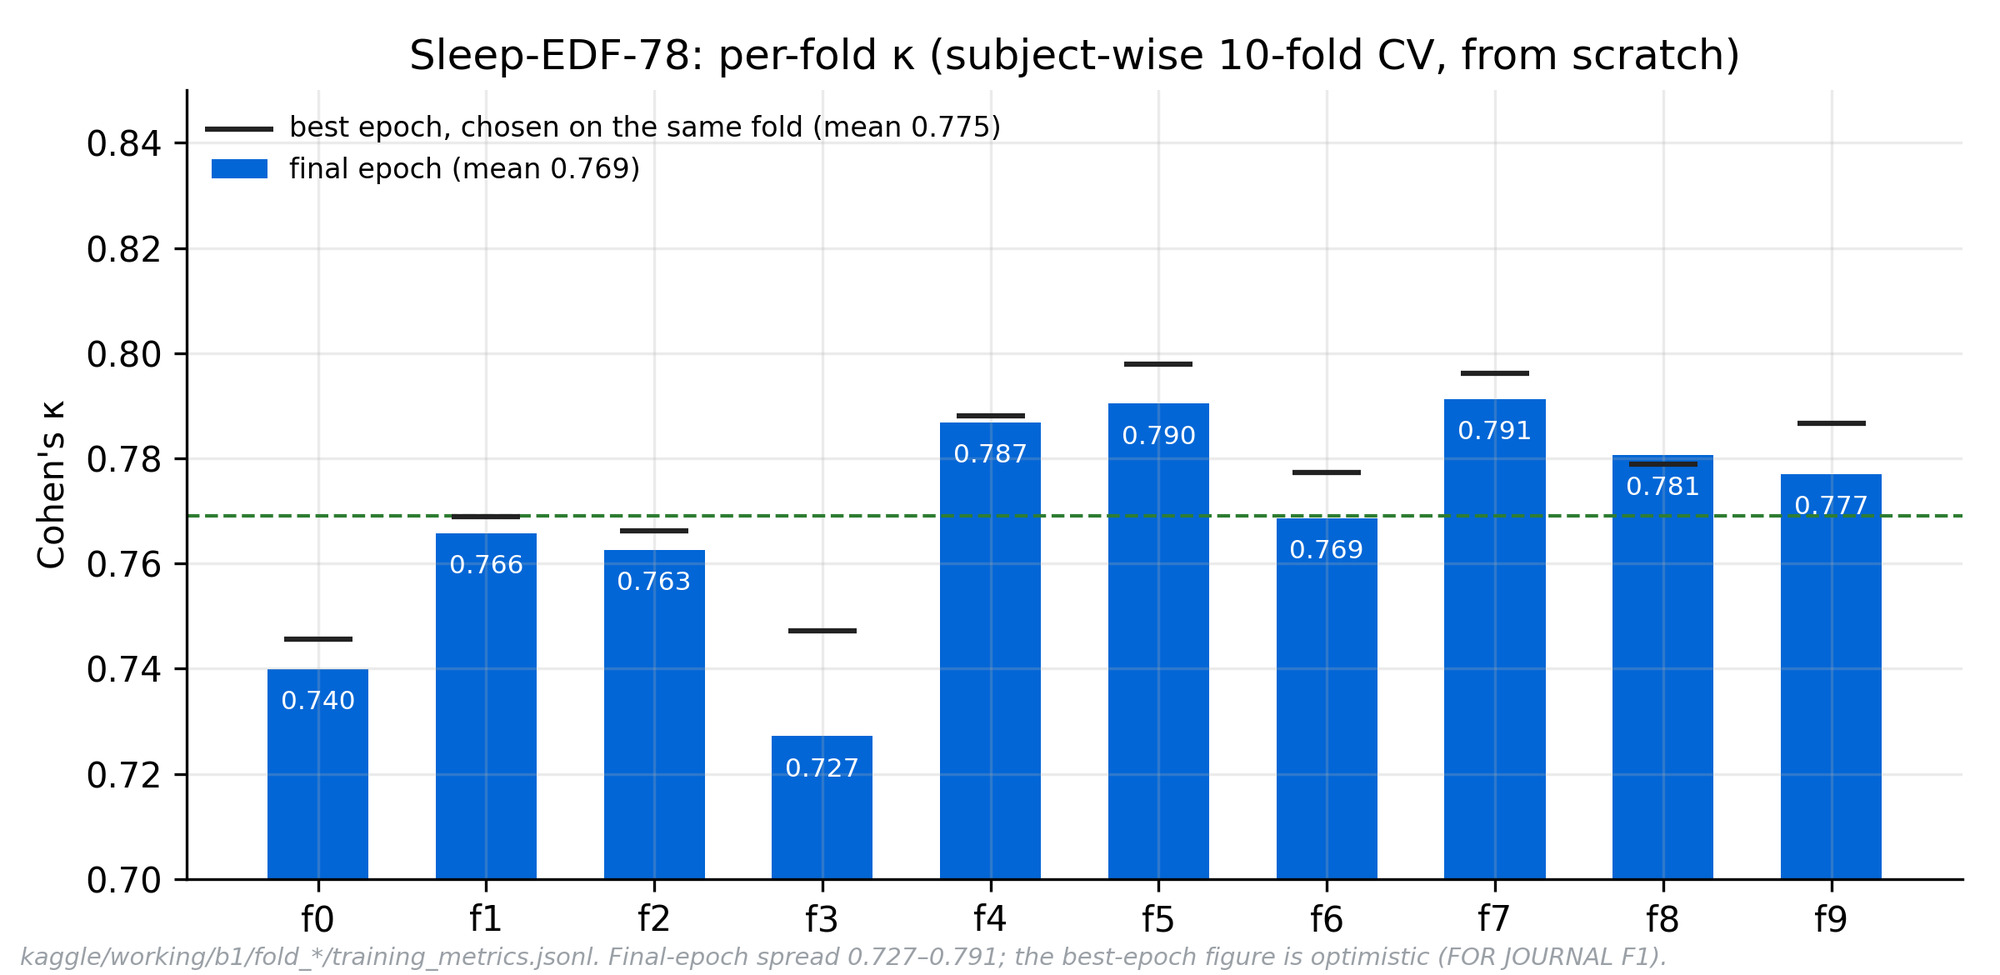
\includegraphics[width=0.85\textwidth]{F17_b1_folds.jpg}
\caption{B1 per-fold $\kappa$ (bars: final epoch, mean 0.769; markers: selected epoch).}
\label{fig:b1folds}
\end{figure}

\begin{figure}[htbp]
\centering
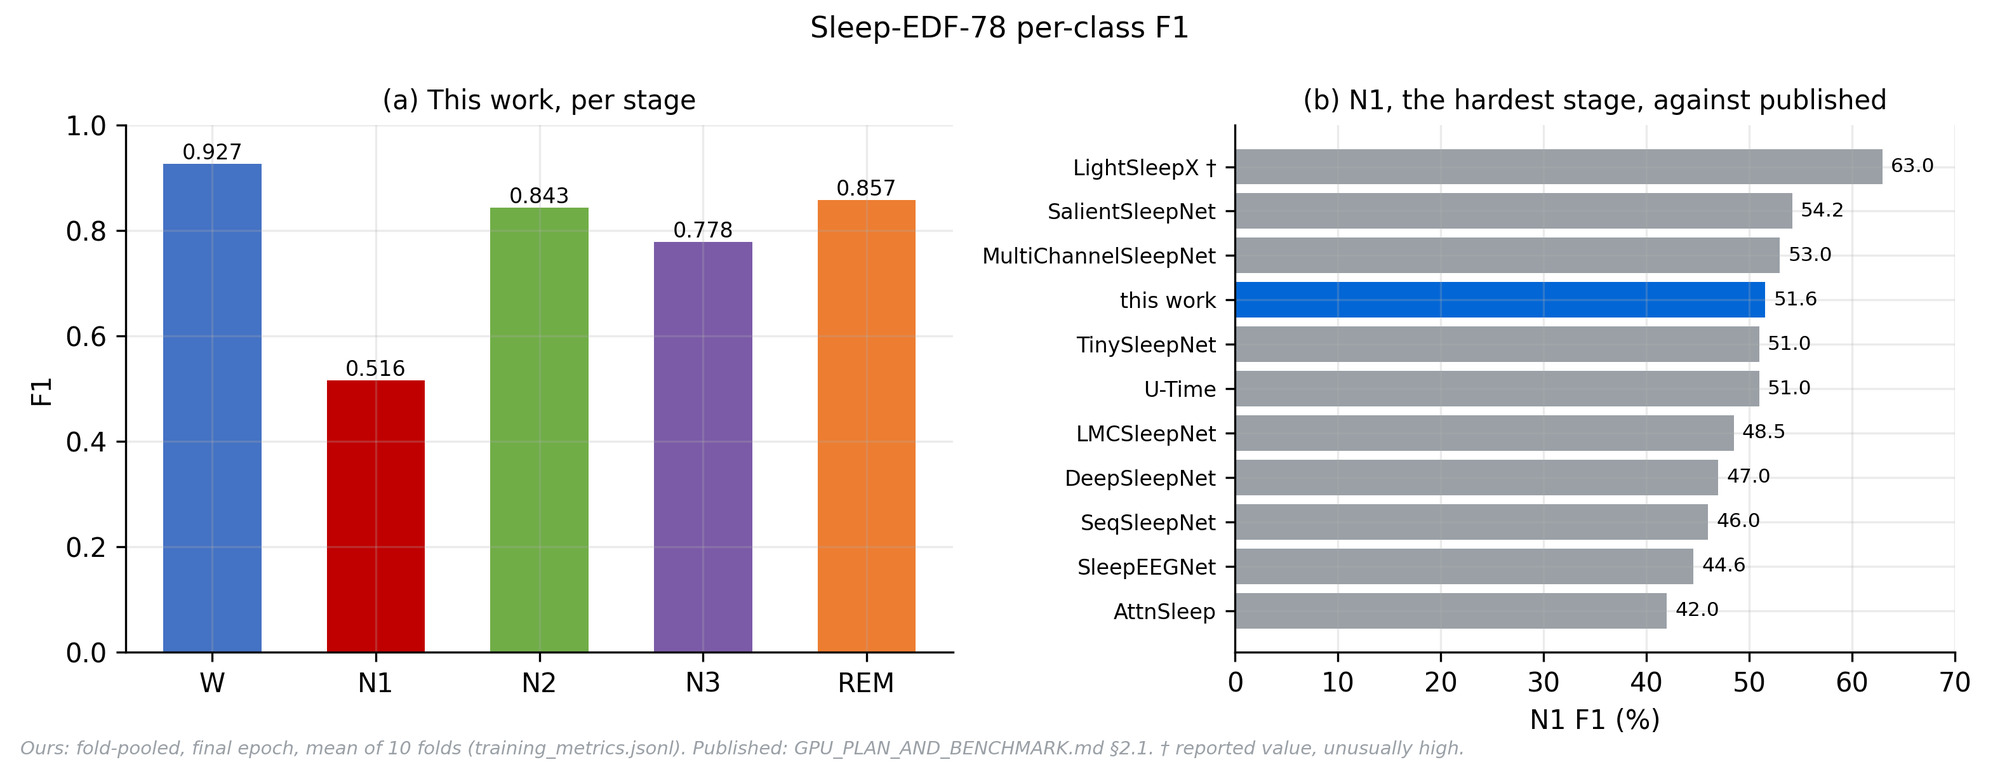
\includegraphics[width=0.85\textwidth]{F19_b1_per_class.jpg}
\caption{B1 per-class F1.}
\label{fig:b1class}
\end{figure}

\subsection{Stage 3 --- Evidence packet (release v2)}

\begin{table}[htbp]
\centering\small
\caption{Calibration and confidence signals of the v2 packet.}
\label{tab:packetres}
\begin{tabularx}{\textwidth}{lY}
\toprule
Signal & Result \\
\midrule
Calibration temperature & 1.0021 (fitted on validation): v2 is already calibrated (EMA, label smoothing) \\
ECE, test & 0.0133 before, 0.0134 after; validation 0.0119 $\rightarrow$ 0.0120 \\
Per-stage reliability (test F1) & W 0.914 high; N2 0.844 high; REM 0.837 high; N3 0.809 high; \textbf{N1 0.507 low} \\
Night confidence vs expert agreement & Test Pearson $r = -0.637$ ($p = 2.0\times10^{-4}$), Spearman $\rho = -0.614$; validation $r = -0.543$ \\
Independent of stage composition & Partial $r = -0.623$ controlling for N1 and REM fraction \\
Tiers (validation-fitted), test mean $\kappa$ & High 0.788 (15 nights) $>$ medium 0.731 (4) $>$ low 0.689 (10): monotone without being fitted on test \\
Triage & Flagging the 10 lowest-confidence nights catches 5 of the 10 worst \\
Derived-metric reliability & 3 robust, 13 fragile, 8 unreliable of 24 (Figure~\ref{fig:reliab}) \\
N1 confidence flag & Threshold 0.475 fitted on validation; not measured on test for v2 \\
\bottomrule
\end{tabularx}
\end{table}

\begin{figure}[htbp]
\centering
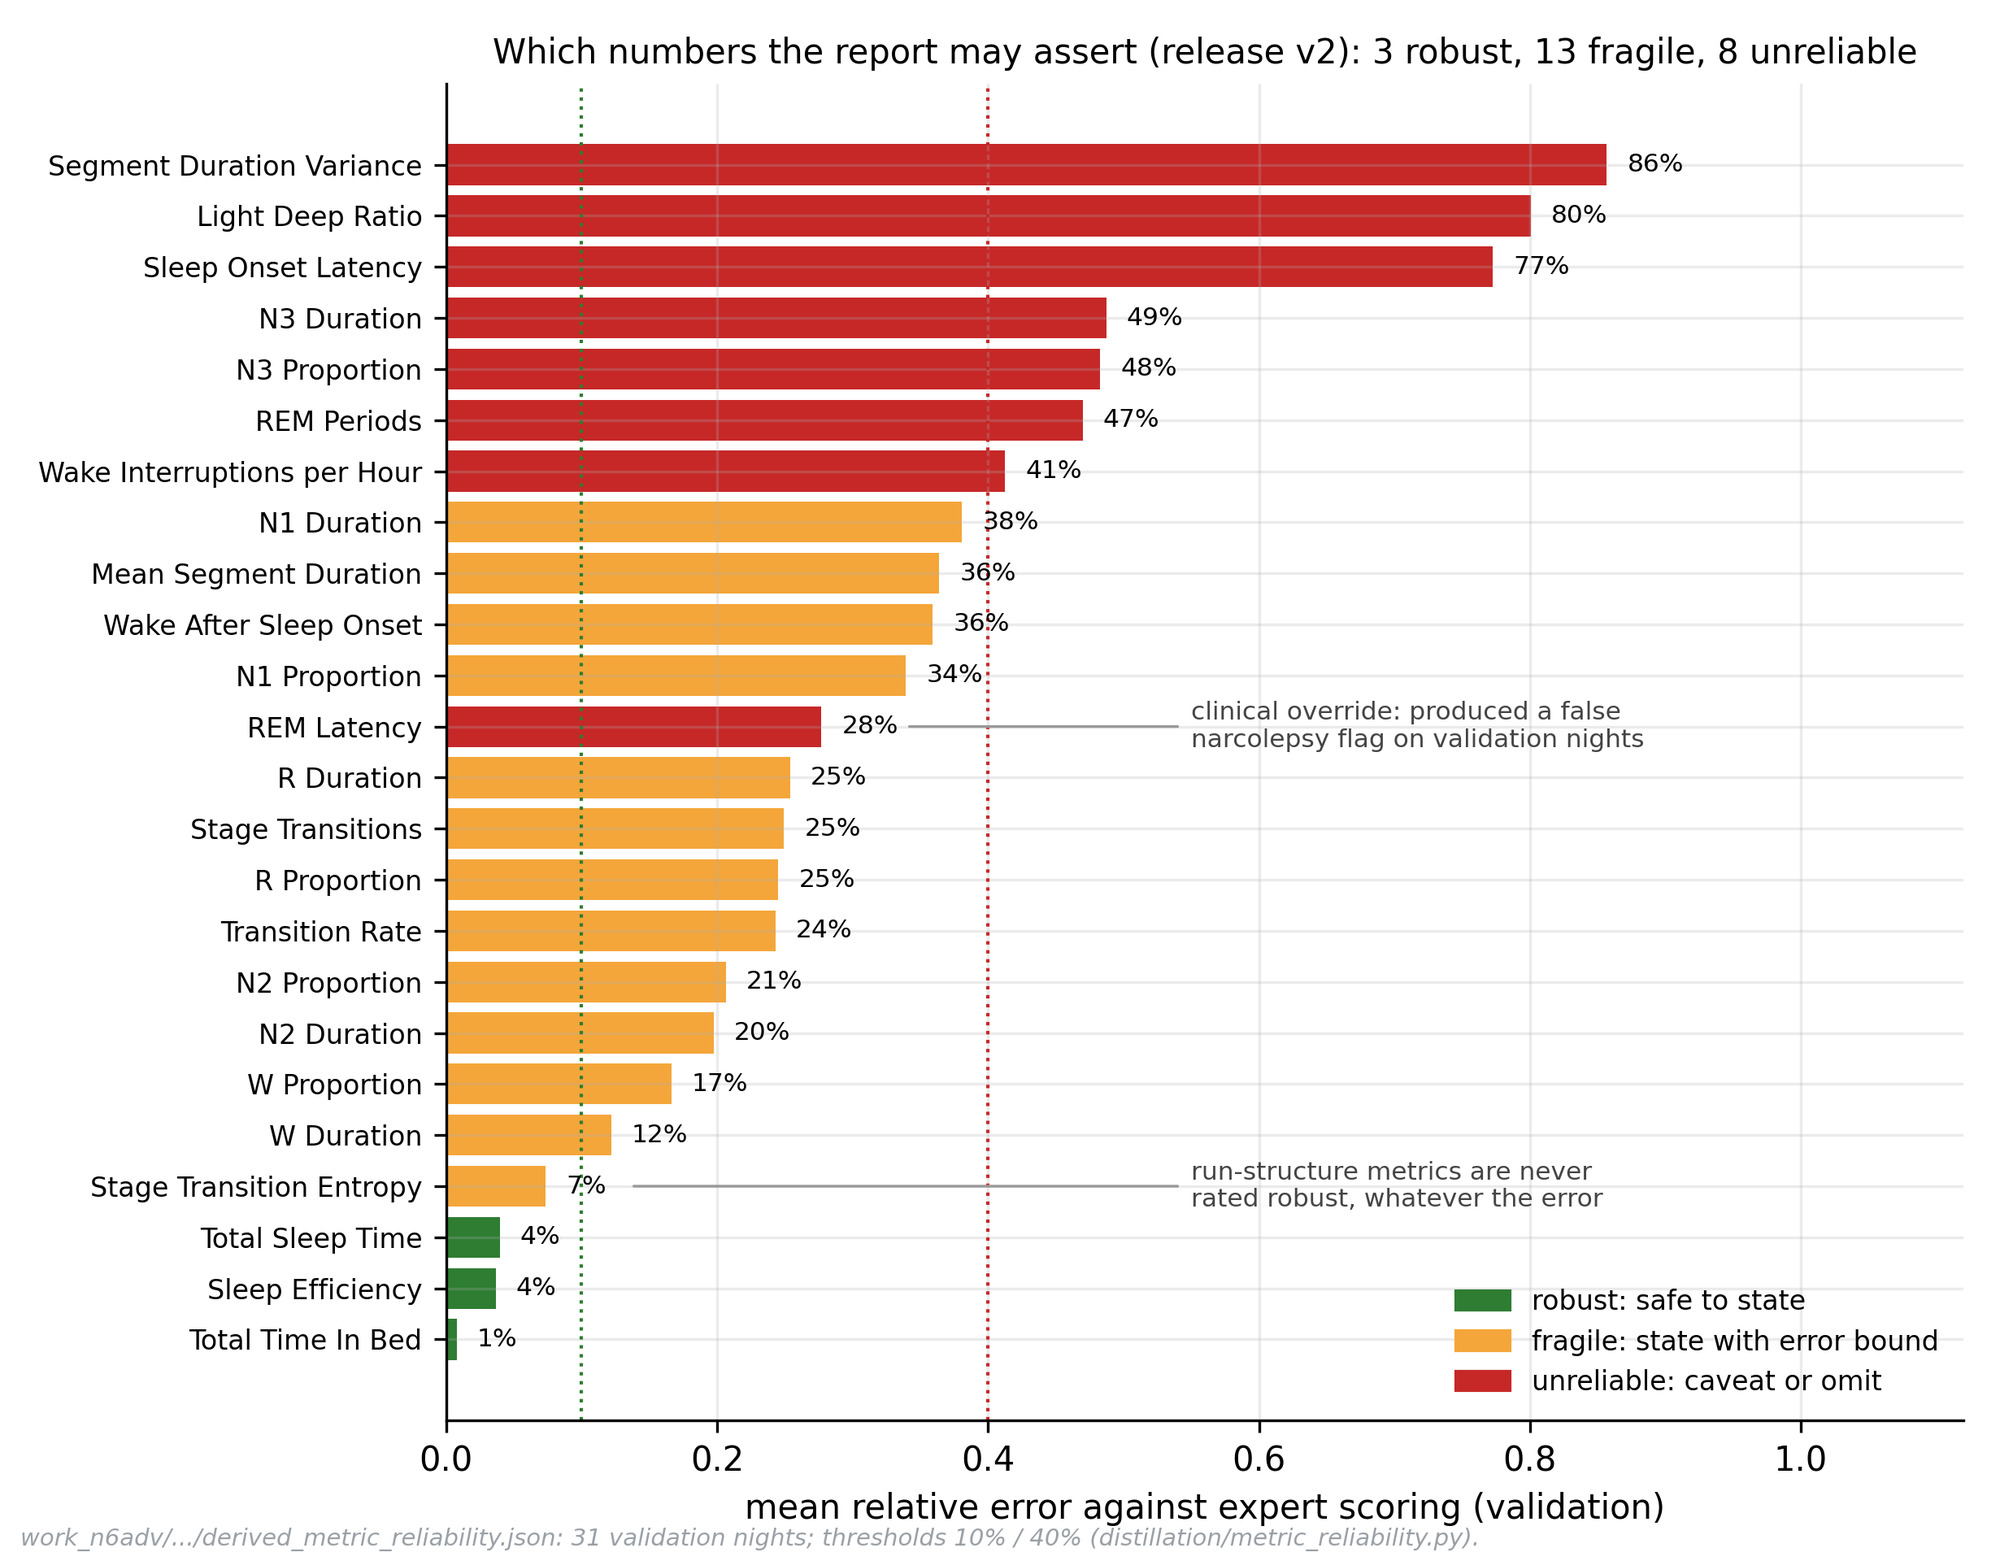
\includegraphics[width=0.85\textwidth]{F30_metric_reliability.jpg}
\caption{Derived-metric reliability: which numbers a report may state.}
\label{fig:reliab}
\end{figure}

\textbf{Plain-language layer.} Clock offsets were reproduced for 168/168 dev and train nights, and the sleep period
used for "awakenings longer than 5 minutes" reproduces each packet's own WASO and sleep-onset latency exactly
(168/168). That awakenings measure turned out to be \emph{unreliable} on v2 (47\% relative error on the 31 dev
nights; within one awakening on 84\% of nights), so it is shown only in the details for a doctor, ungraded. A
second finding: the packet reports stages as a share of the whole recording, while clinical norms use share of
sleep time, so norms are compared only against the latter.

\subsection{Stage 4 --- Small language model}

\textbf{Is the contract achievable?} A large reference model (Gemini 3.1 Flash, temperature 0, structured output +
grammar, prompt P1) produced 30/30 reports at 5/5 with 0 violations and numeric fidelity 1.000 on dev. Its
verifier-passing outputs on the 123 training nights became the training targets.

\textbf{Do untrained small models need training?} With the grammar, the five candidates (Qwen2.5-1.5B,
SmolLM2-1.7B, Gemma-2-2B, Llama-3.2-3B, Phi-3.5-mini) reached 0, 0, 0, 2 and 0 of 31 at 5/5; without it, 0/31 each.
The grammar secures syntax, not meaning; no base model knows the contract.

\begin{table}[htbp]
\centering\small
\caption{Report-model selection (pre-registered bar: $\ge$25/31 at 5/5 on dev).}
\label{tab:slm}
\begin{tabularx}{\textwidth}{lrrrrY}
\toprule
Model & Dev 5/5 & Dev viol. & Test 5/5 & Test viol. & Notes \\
\midrule
Llama-3.2-3B base & 2/31 & -- & -- & -- & Untrained \\
Qwen-Student 1.5B & 10/31 & 0 & 12/29 & 0 & Misses about 1 of 5 items; capacity limit \\
Llama-Student v1 (v1 packets) & 30/31 & 3 & 29/29 & 0 & Fidelity 1.000; peak RAM 4,719 MiB \\
\textbf{Llama-Student v2 (current)} & \textbf{31/31} & \textbf{0} & \textbf{28/29} & 2 (blocked) & Dev fidelity 527/527; test 492/493; \textbf{0 flawed released} \\
\bottomrule
\end{tabularx}
\end{table}

v1 and v2 were scored on different packets and are reported side by side, never pooled (Fisher's exact $p = 1.0$
for the one-night difference). 95\% lower bounds: v1 test $\ge$88.1\%, v2 dev $\ge$88.8\%, \textbf{v2 test
$\ge$82.2\%} (Table~\ref{tab:slm}, Figure~\ref{fig:reports}).

\textbf{The one blocked night (SC4611E0).} REM is 0.12\% of that night, so the packet's sustained-REM latency is
\texttt{None}. The model wrote $-1.0$ instead of omitting the claim. The verifier flagged \texttt{L2.value\_mismatch}
and \texttt{L2.uncited\_quantity}, the text was never rendered, and the agent delivered the fallback summary --- the
system working as designed.

\begin{table}[htbp]
\centering\small
\caption{Verifier ablation on 31 dev nights: reports released with a flaw (definitions pre-registered).}
\label{tab:verabl}
\begin{tabular}{lrrr}
\toprule
Report model & Gate on & Gate off & Gate and grammar off \\
\midrule
\textbf{Llama-Student v2} (v2 packets) & \textbf{0/31} & \textbf{0/31} & \textbf{0/31} \\
Llama-Student v1 (v1 packets) & 0/31 & 1/31 & 2/31 \\
Llama-3.2-3B base (v1 packets) & \textbf{0/31} (all fall back) & 31/31 & 31/31 \\
\bottomrule
\end{tabular}
\end{table}

With the grammar removed, v2's output was byte-identical to its constrained output on all 31 nights: at temperature
0 the grammar never changed a token (Table~\ref{tab:verabl}, Figure~\ref{fig:verabl}). For the fine-tuned model the
verifier is a safety net (it blocked 1 of 29 on test); for an untrained model it is decisive.

\textbf{Determinism.} Llama's chat template wrote today's date into the prompt, so outputs changed from day to day;
pinning the template to the training date fixed it. \texttt{llama-server} did not reproduce the evaluated outputs
(20--23/31 vs 30/31), so the system uses one-shot \texttt{llama-completion}.

\begin{figure}[htbp]
\centering
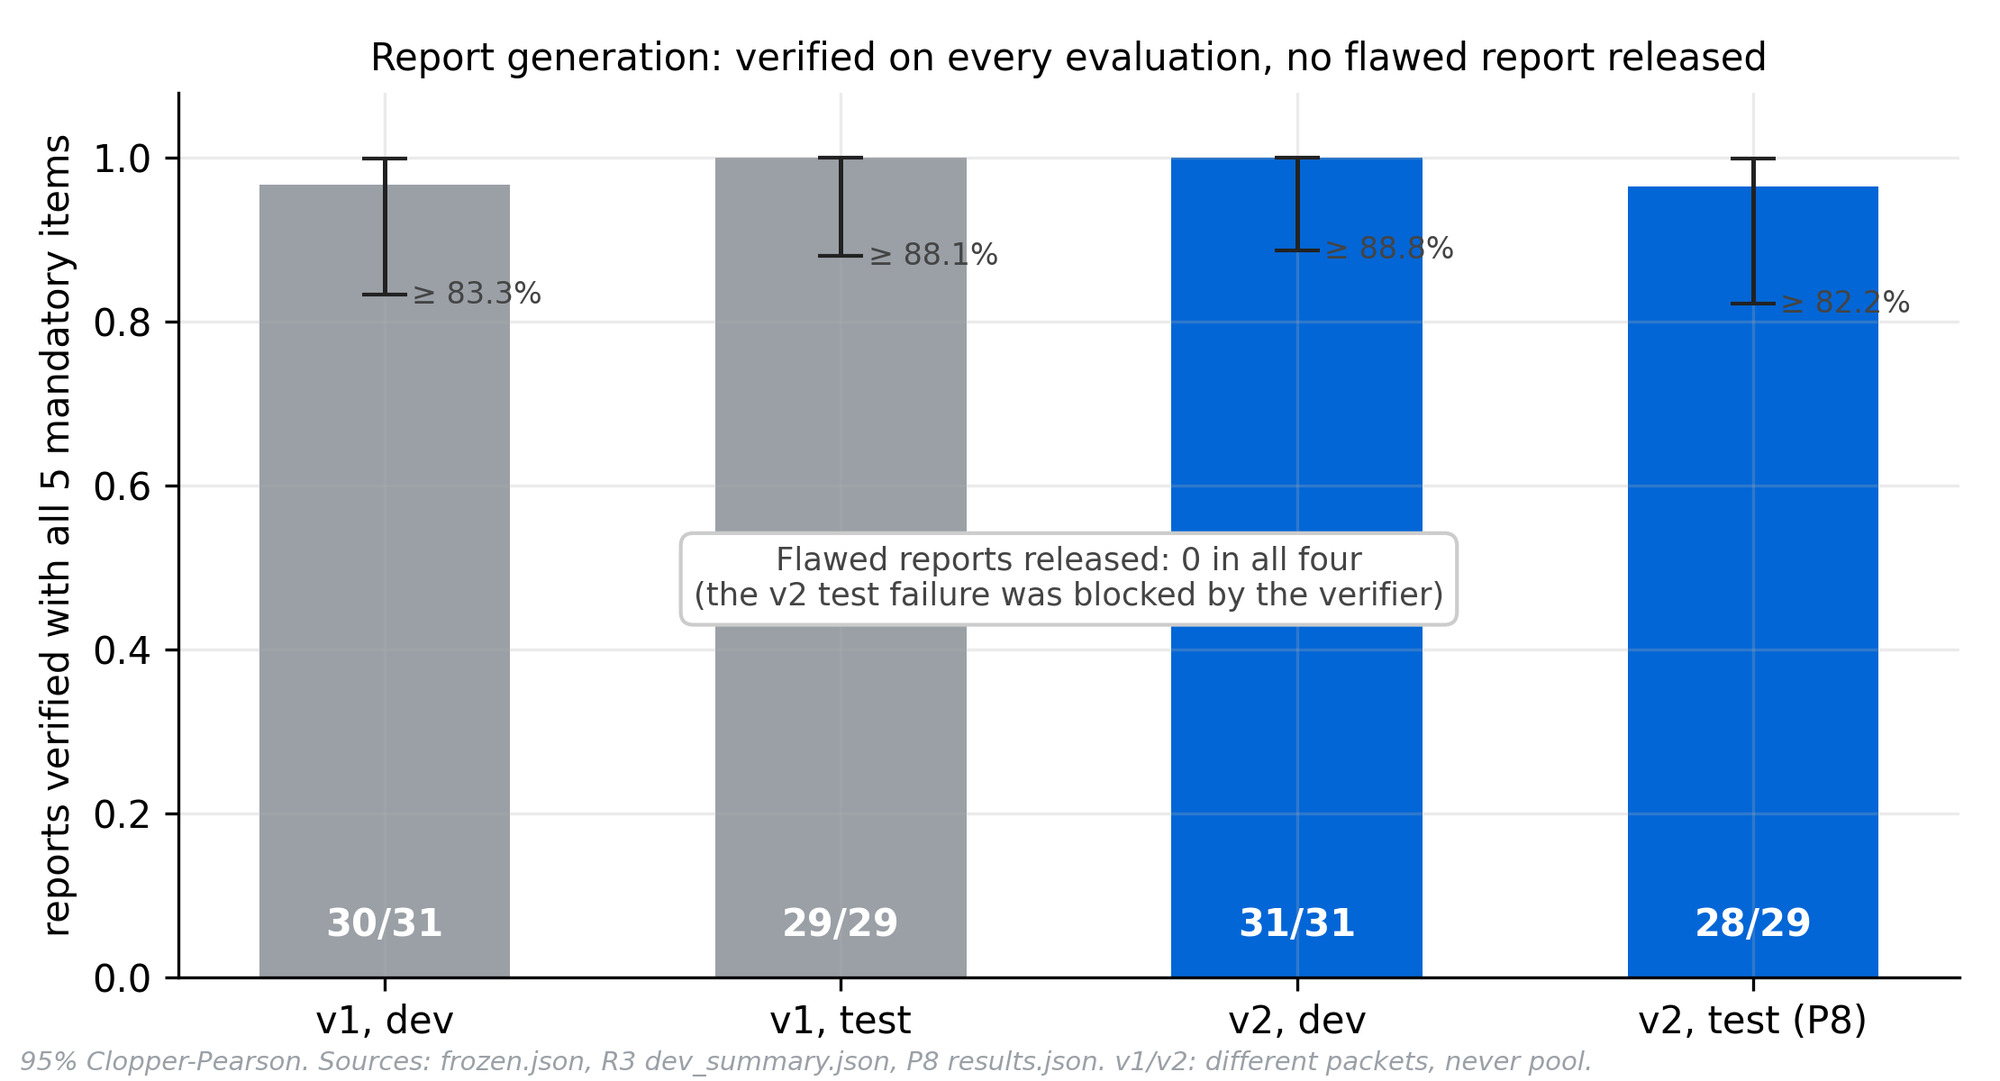
\includegraphics[width=0.85\textwidth]{F25_report_verification.jpg}
\caption{Report verification across releases and splits, with 95\% Clopper--Pearson intervals; 0 flawed reports released in all four.}
\label{fig:reports}
\end{figure}

\begin{figure}[htbp]
\centering
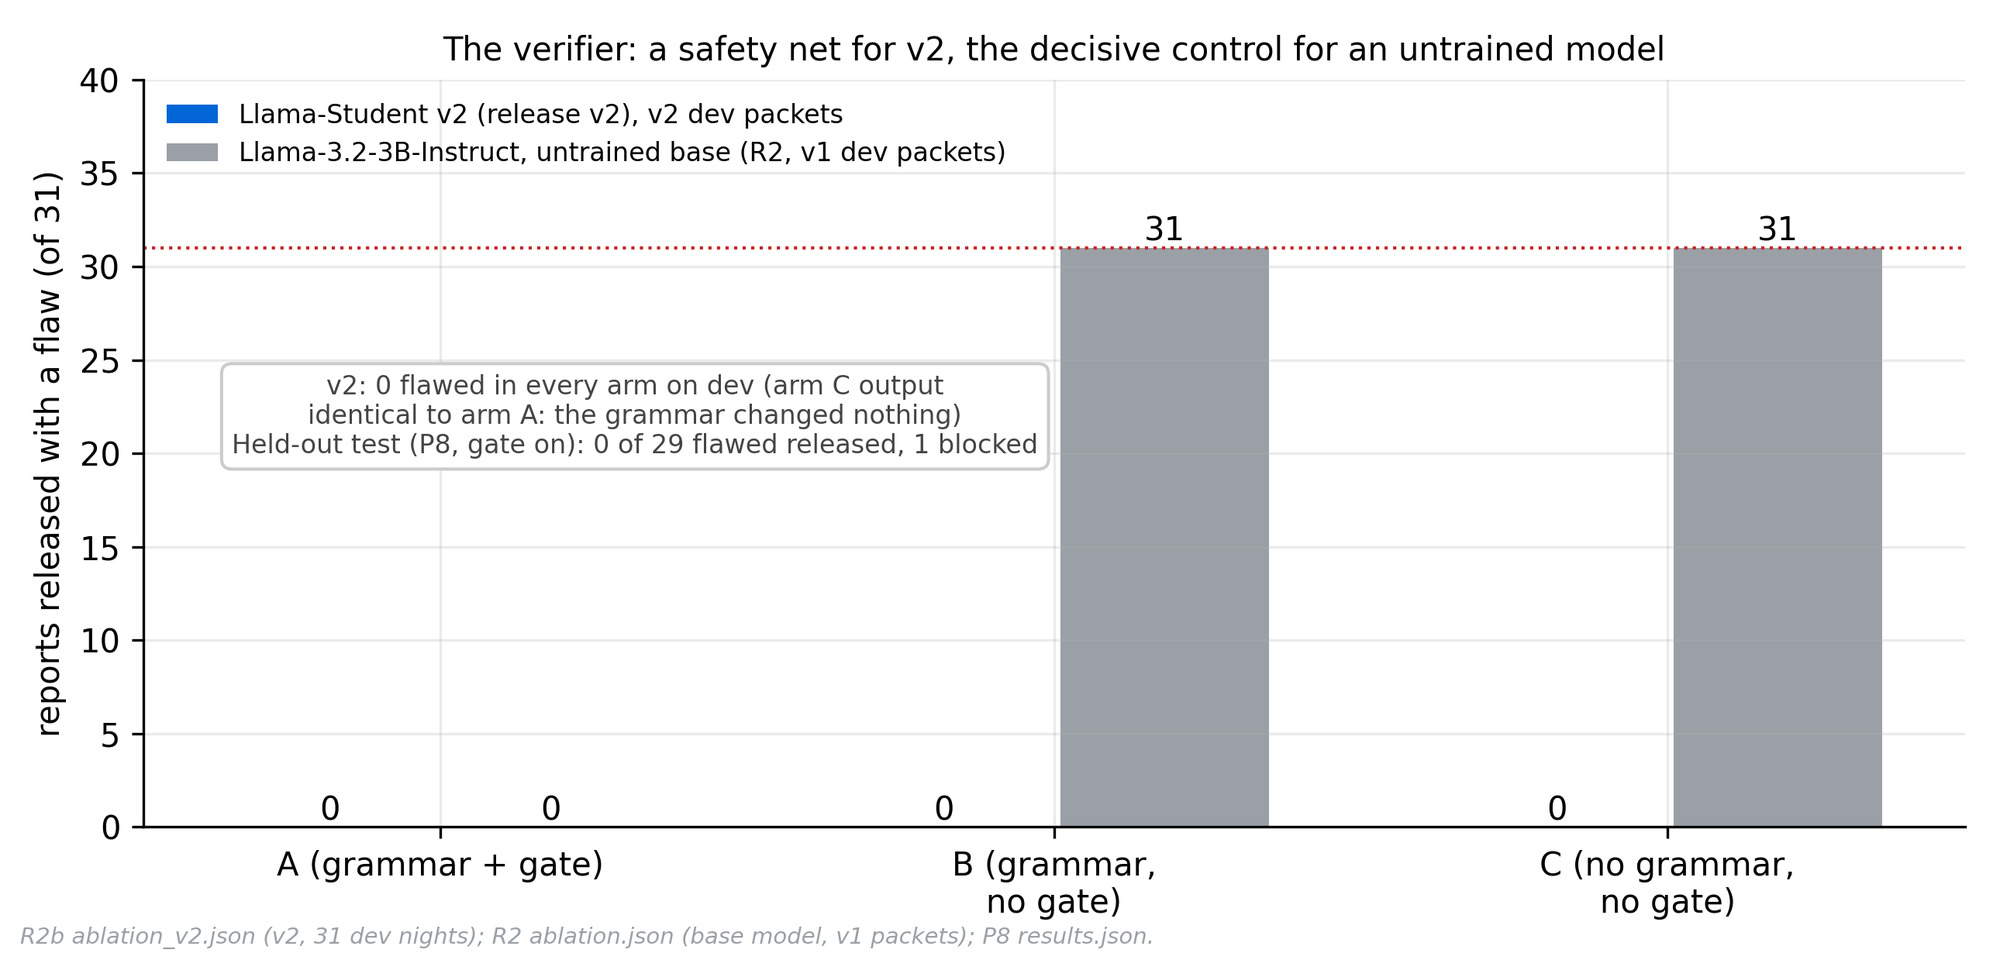
\includegraphics[width=0.85\textwidth]{F20_verifier_ablation.jpg}
\caption{Verifier ablation: flawed reports released with and without the gate.}
\label{fig:verabl}
\end{figure}

\subsection{Stage 5 --- Agentic workflow}

\begin{table}[htbp]
\centering\small
\caption{Fault scenarios (real EDF files from a dev night; injected report-model faults).}
\label{tab:faults}
\begin{tabular}{llll}
\toprule
\# & Scenario & Expected outcome & Result \\
\midrule
S01 & Clean night, no hypnogram & VERIFIED\_REPORT & \yes \\
S02 & Prebuilt packet (Path A) & VERIFIED\_REPORT & \yes \\
S03 & EEG flat for 2\,h & REVIEW\_ONLY Q01 & \yes \\
S04 & EOG missing & VERIFIED\_REPORT & \yes \\
S05 & Fpz-Cz missing, Pz-Oz present & REVIEW\_ONLY W05 & \yes \\
S06 & Recorded at 128\,Hz & VERIFIED\_REPORT (resampled) & \yes \\
S07 & Only 2\,h recorded & REJECTED R03 & \yes \\
S08 & Corrupt header & REJECTED R01 & \yes \\
S09 & Report model crashes once & VERIFIED\_REPORT after retry & \yes \\
S10 & Report model hangs & FALLBACK F02 & \yes \\
S11 & Report model writes invalid claims & FALLBACK F03 & \yes \\
S12 & Device at 82\,$^\circ$C & FALLBACK F01 after 12 waits & \yes \\
S13 & Power cut during generation & VERIFIED\_REPORT, one delivery & \yes \\
S14 & Strong 49\,Hz line noise & VERIFIED\_REPORT at the time & \yes; led to the Q03 check \\
S15 & Two nights of one subject (trend) & -- & deferred (needs history store) \\
\bottomrule
\end{tabular}
\end{table}

\textbf{14/14 pass, 1 deferred} (Table~\ref{tab:faults}). The invariants hold on every run: I1 no unverified text;
I2 every number has provenance; I3 frozen components; I4 no network; I5 expert hypnograms never read by the
workflow; I6 every run ends; I7 every step traced; I8 every failure visible in the review queue. Crash recovery at
eight boundaries produced exactly one delivery each time.

\begin{table}[htbp]
\centering\small
\caption{Further robustness results.}
\label{tab:robust}
\begin{tabularx}{\textwidth}{lY}
\toprule
Check & Result \\
\midrule
Real recordings end to end (Path B, v2, 31 dev nights) & Mean per-night $\kappa$ 0.701 (v1 0.673; v2 higher on 27/31); pooled accuracy 79.5\%, $\kappa$ 0.719; \textbf{30 verified + 1 sent to review (line noise)}; median 78\,s per report on x86 \\
Night boundaries without an expert & Start: median 0, p90 2 epochs; end: median 2, p90 41 epochs (bar 30; accepted deviation) \\
Sampling rates (3 nights $\times$ 2 releases $\times$ 128/256\,Hz) & 18/18 outcomes match 100\,Hz; hypnogram agreement 0.992--1.000 \\
Line noise & A 49\,Hz tone at 1$\times$ EEG RMS drops $\kappa$ 0.775 $\rightarrow$ 0.340, and the verifier cannot see it, so an input check (Q03/W10) was added \\
Quality flags predict worse staging & Dev nights flagged W02: $\Delta\kappa$ $-0.138$, 95\% CI [$-0.202$, $-0.072$] \\
Reproducibility (real model, 2 runs $\times$ 31 nights) & 31/31 byte-identical report pages \\
Preprocessing parity with training & 31/31 exact (EEG, 34 features, probabilities) \\
\bottomrule
\end{tabularx}
\end{table}

\begin{figure}[htbp]
\centering
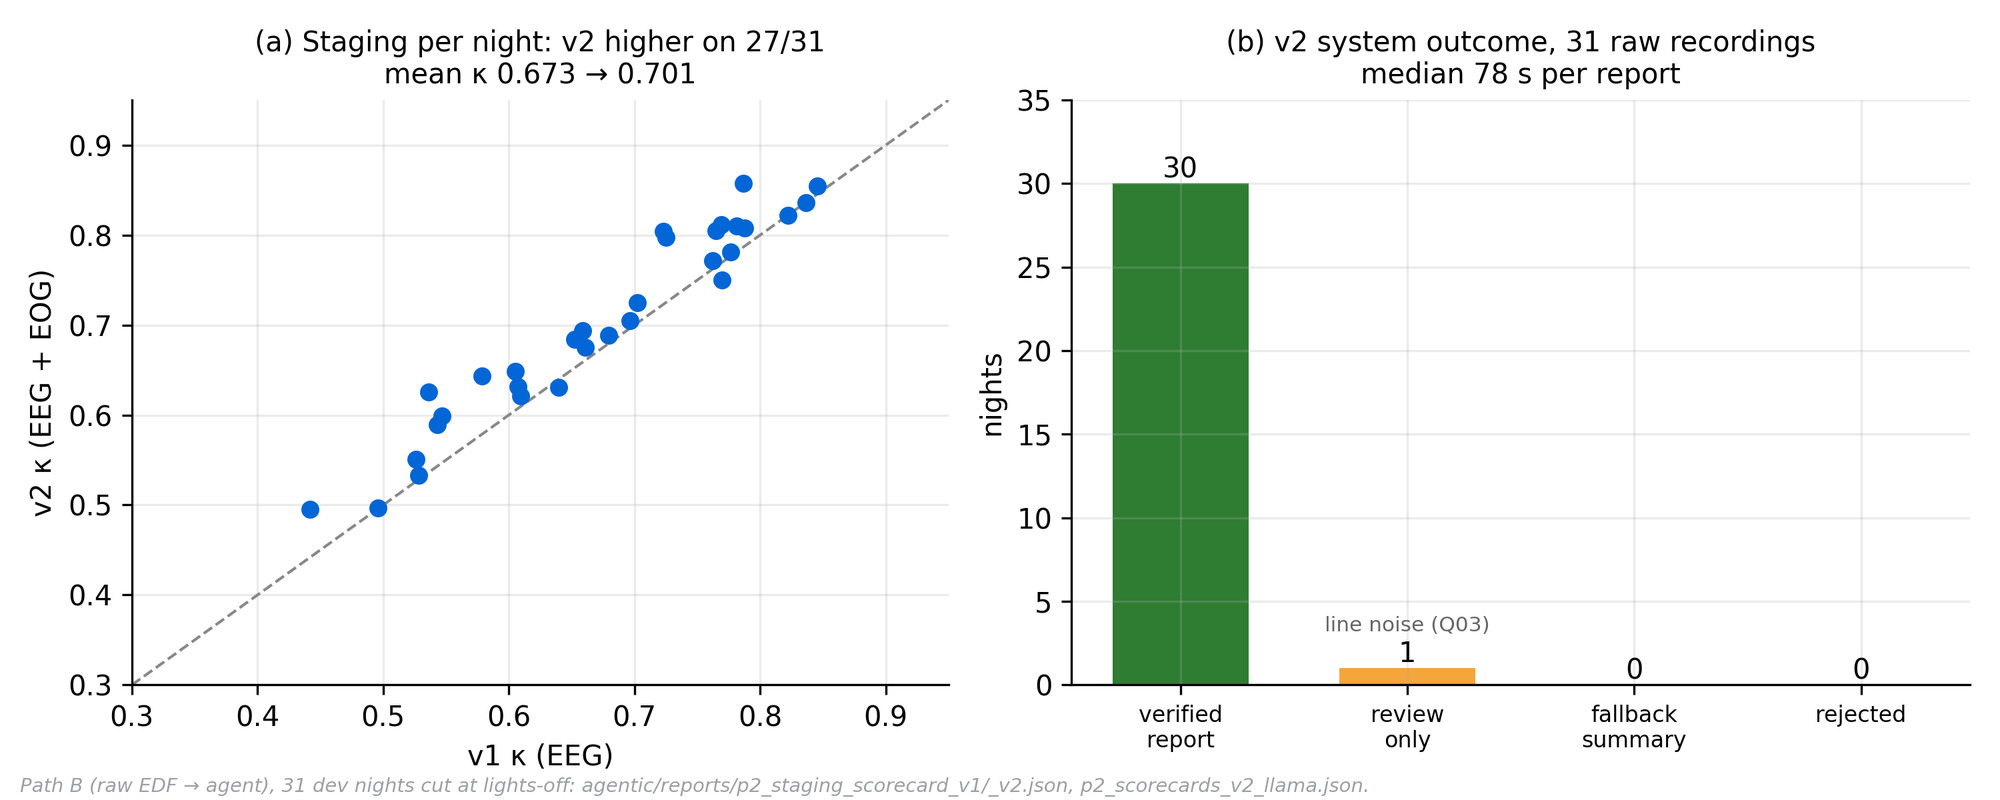
\includegraphics[width=0.85\textwidth]{F29_real_recordings.jpg}
\caption{Real recordings end to end (Path B): v2 against v1 per night.}
\label{fig:pathb}
\end{figure}

\begin{figure}[htbp]
\centering
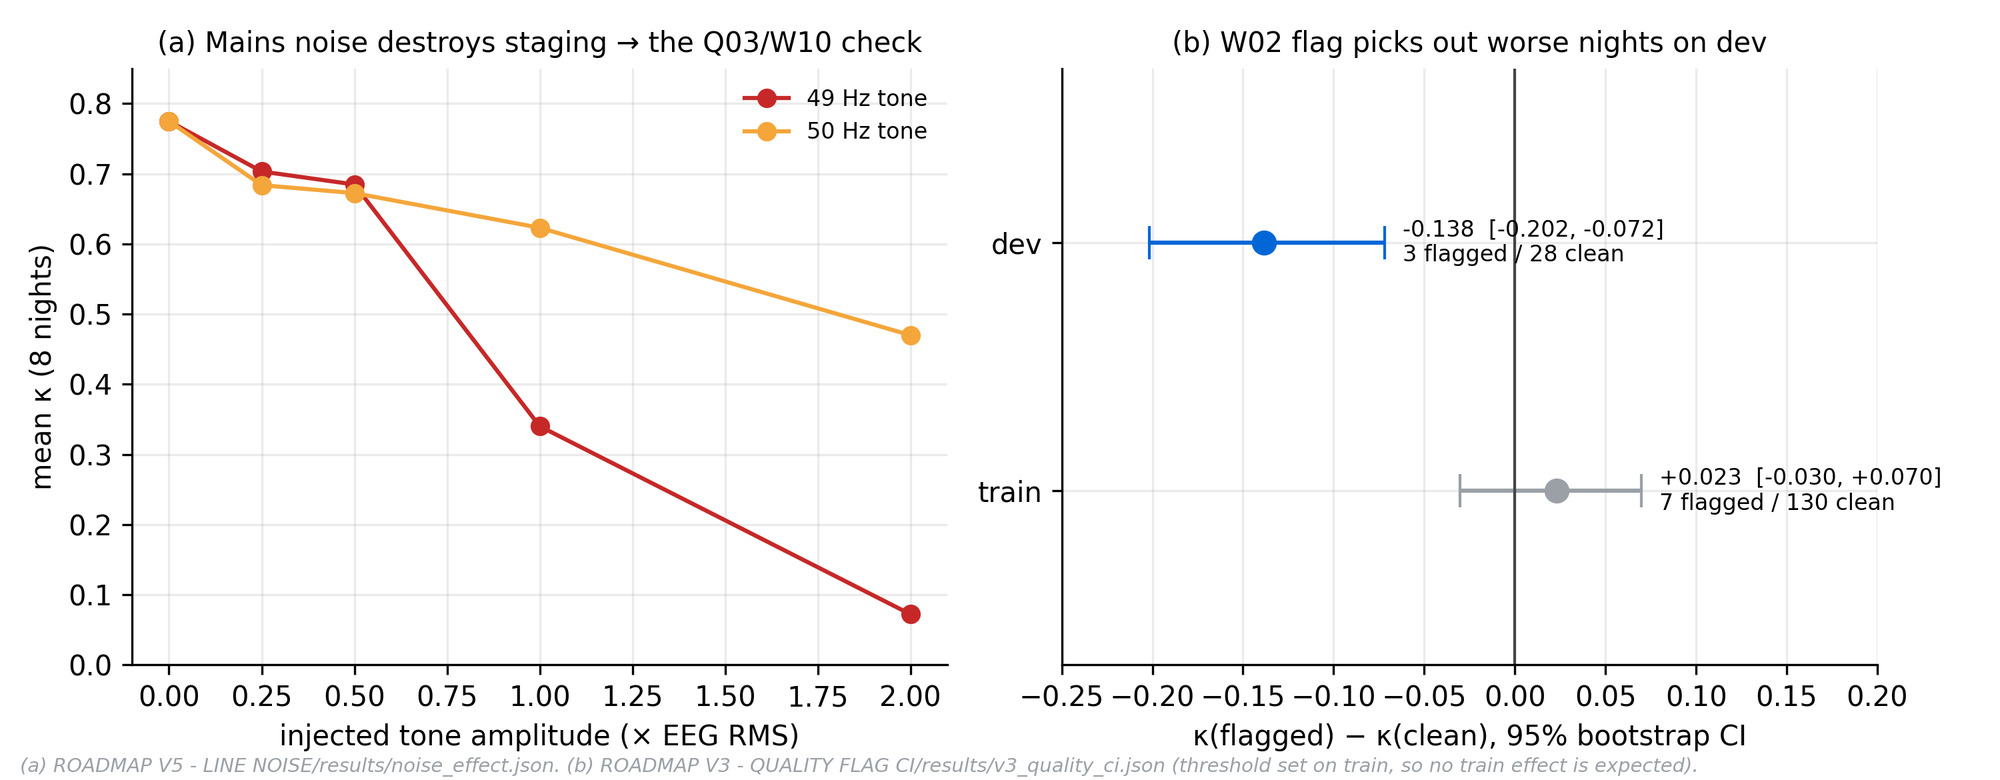
\includegraphics[width=0.85\textwidth]{F31_quality_checks.jpg}
\caption{Signal-quality checks and the effect of line noise.}
\label{fig:quality}
\end{figure}

\begin{figure}[htbp]
\centering
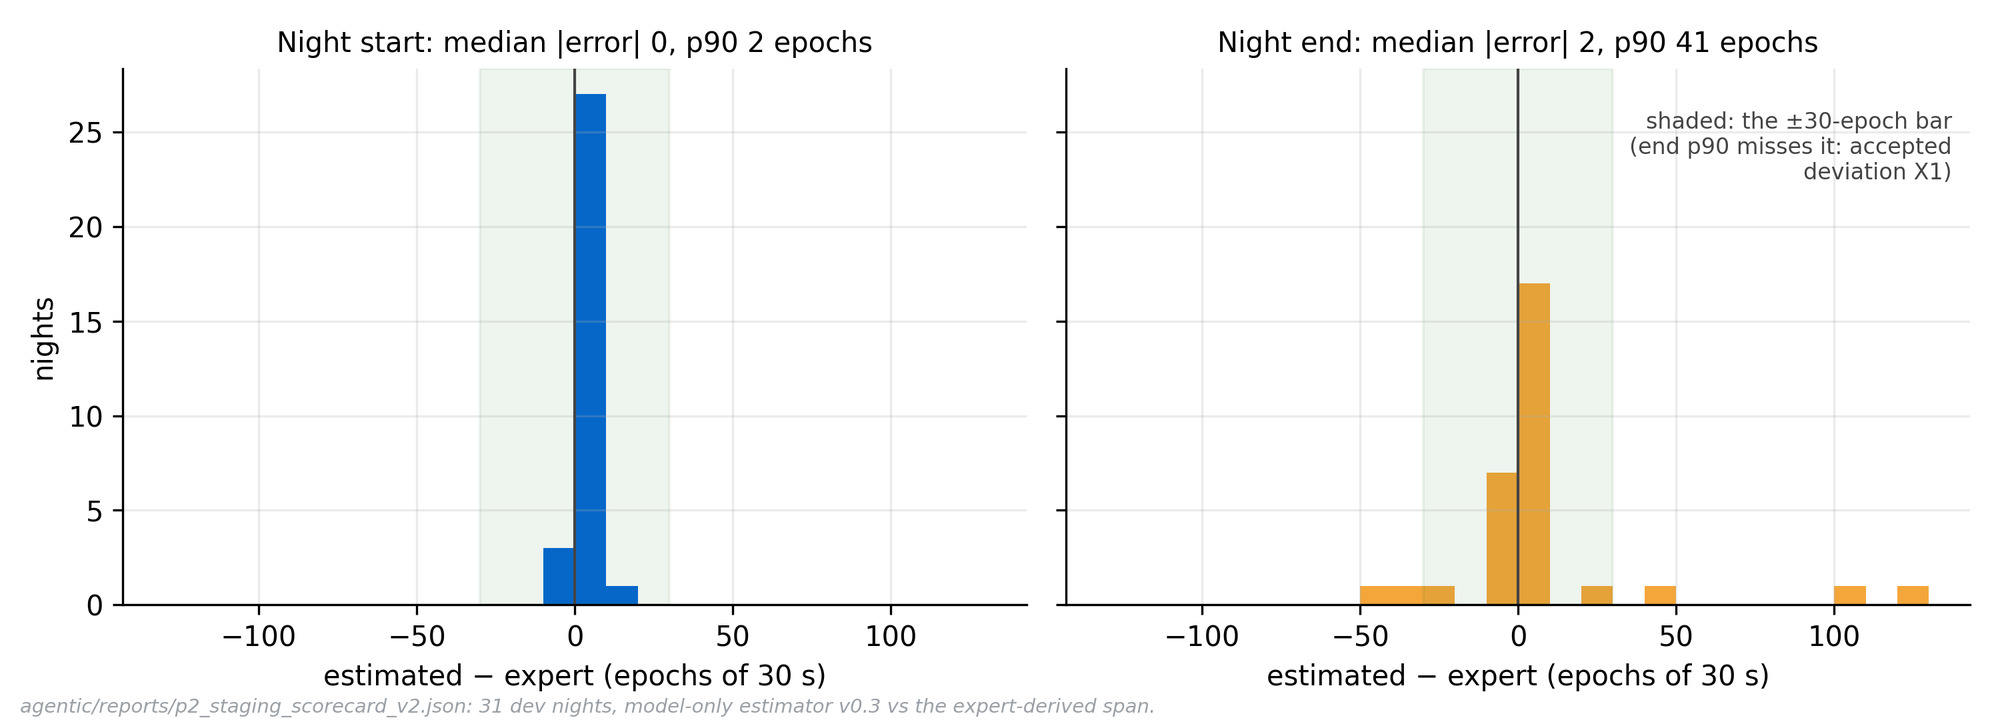
\includegraphics[width=0.85\textwidth]{F32_night_boundaries.jpg}
\caption{Night boundaries found without an expert.}
\label{fig:bounds}
\end{figure}

\subsection{Stage 6 --- Edge-device simulation (Raspberry Pi 5, 16\,GB)}

\textbf{L1 and L2: offline containers limited like the Pi.} The agent ran unchanged in a Linux x86-64 Docker container
(4 CPUs, 16\,GiB, \texttt{--network none}, project and data read-only, llama.cpp b10927 compiled inside the image) on a
second Windows PC (Table~\ref{tab:l1}). The cgroup limits were confirmed from inside the container. The first run of
this experiment exposed three faults in the container bundle (missing llama.cpp shared libraries, a missing module and a
zip step); they were fixed and the experiment repeated, and only the repeated run is reported. In it:
\begin{itemize}
  \item Staging on all 31 raw dev recordings matched the Windows reference run exactly at the hypnogram level, with
  probability differences more than five times below the acceptance bar.
  \item The report model, run on all 31 evidence packets, produced 31/31 verified reports whose text was
  \textbf{byte-identical} to the reference PC's, at a median of 151\,s per report and a peak of 5.16\,GB for the whole
  process tree. The three-night end-to-end run (raw EDF to delivered page) reproduced the reference outcome on all three;
  the night the reference run sent to review (SC4111E0, line noise, Q03) was sent to review again.
  \item Under ARM64 emulation (QEMU), the staging stage on 8 nights gave identical hypnograms with a maximum probability
  difference of $7.7\times10^{-7}$. The emulated run was seven times slower (133\,s against 18\,s per night), which
  is a property of the emulation and not a timing of the Pi.
\end{itemize}
These are x86 timings on a desktop CPU; they bound nothing about the Pi's speed. They do show that the whole release
runs, offline and verified, inside the memory the Pi has, and that its output does not depend on the operating system or
compiler.

\begin{table}[htbp]
\centering\small
\caption{Edge simulation in Docker (4 CPUs / 16\,GiB / no network): x86-64 and ARM64 under emulation.}
\label{tab:l1}
\begin{tabularx}{\textwidth}{lYl}
\toprule
Check & Result & Verdict \\
\midrule
P1 no network & TCP to 1.1.1.1:53 and DNS lookup both blocked & \textbf{met} \\
P4 no secrets in the image & No \texttt{.env}, no API-key pattern in the mounted project or the image & \textbf{met} \\
Release pins & All pinned hashes match inside the container; \texttt{llama-completion} starts & \textbf{met} \\
Staging parity, Linux x86 vs reference PC & 31/31 nights, 61/61 arrays (pass 1 + pass 2) with identical hypnograms; max $|\Delta p| = 1.8\times10^{-5}$ (bar $10^{-4}$) & \textbf{met} \\
Report model, 31 dev packets (Path A) & 31/31 VERIFIED\_REPORT; text identical to the reference on 31/31; median 151\,s, p95 160\,s; peak 5.16\,GB & \textbf{met} \\
End to end, 3 raw nights (Path B) & Outcome equals the reference on 3/3 (2 verified, SC4111E0 review Q03); staging max $|\Delta p| = 8.3\times10^{-7}$; median 158\,s; peak 5.64\,GB & \textbf{met} \\
E1 staging parity on ARM64 (QEMU), 8 SC nights & 15/15 arrays with identical hypnograms; max $|\Delta p| = 7.7\times10^{-7}$ & \textbf{met in emulation} \\
Not yet run & ARM report model; ST nights on ARM; Raspberry Pi 5 timing, heat and power; 7-night soak & open \\
\bottomrule
\end{tabularx}
\end{table}

\begin{table}[htbp]
\centering\small
\caption{Per-night budget on the Raspberry Pi 5 (analytical estimates, not measurements).}
\label{tab:budget}
\begin{tabular}{lr}
\toprule
Step & Estimate \\
\midrule
Ingest + quality checks & 5--20\,s \\
Study period (two-pass staging) & 5--15\,s \\
Preprocess (resample, epochs, 34 features) & 10--40\,s \\
Staging (175\,K params, CPU) & 2--10\,s \\
Packet & $<$5\,s \\
Report prefill ($\sim$1,100 tokens at an assumed 15--30 tokens/s) & 40--80\,s \\
Report generation ($\sim$1,200 tokens at 3.06--4.37 tokens/s; ceiling 7.43) & 266--380\,s \\
Verifier + render & $<$2\,s \\
\midrule
\textbf{Total per night} & \textbf{$\approx$6--9 min} (x86 measured: median 78\,s per report native, 151\,s in the 4-CPU container) \\
\textbf{Peak memory} & \textbf{$\approx$6--8\,GB} of 16\,GB (measured in the x86 container: 5.2\,GB report, 5.6\,GB end to end) \\
\bottomrule
\end{tabular}
\end{table}

Memory bandwidth, not memory size, sets the speed (Table~\ref{tab:budget}): the 16\,GB board is not faster than the
8\,GB one, but it keeps every model resident with the full context. \textbf{Pre-registered acceptance bars for the
Pi:} staging parity max $|\Delta p| \le 10^{-4}$ with identical hypnograms (E1); dev 5/5 not below the x86 result,
with every failure caught by the verifier; P95 $\le$15 min per night; peak $\le$10\,GB; no thermal throttling with
the Active Cooler at 25\,$^\circ$C; all fault scenarios and a 7-night unattended soak with 0 crashes. In the container the
parity, report-parity and peak-memory bars are met; the time, heat and soak bars need the device.

\section{ Analysis of Results}

\begin{itemize}
  \item \textbf{Measurement before modelling.} The largest single change in the project came from evaluation, not
  architecture: subject leakage inflated $\kappa$ by about 0.16, and misaligned labels cost about 3 accuracy points.
  Every later result depends on fixing both.
  \item \textbf{Distillation works only with a better teacher.} The negative KD result has a mechanism, and the fix
  (an ensemble of comparable, diverse students) followed from it. Distillation's lasting benefit was calibration,
  which the packet then turns into usable confidence.
  \item \textbf{EOG helps where expected.} Like for like, EOG adds +0.018 $\kappa$, with the gains on N1 and REM,
  the stages defined partly by eye movements; without EOG the model still beats v1.
  \item \textbf{Trust signals are real.} Night confidence ranks nights by agreement with the expert on test without
  being fitted there, and it is not a proxy for stage composition.
  \item \textbf{Training, not the grammar, made the report model correct.} The grammar fixes syntax; fine-tuning
  supplied the semantics; the verifier is the safety net that caught the one remaining error on test.
  \item \textbf{The agent turns failure into a truthful outcome.} Every fault produced a defined page; no scenario
  produced a wrong report.
  \item \textbf{The system is portable.} Moved to Linux, in a container with no network and Pi-like limits, the
  staging stage produced the same hypnograms on every night, and the report model reproduced the reference text
  byte for byte on all 31 packets. The same staging code gave identical hypnograms when run for ARM64 under emulation.
\end{itemize}

\section{Observations:}

\begin{itemize}
  \item \textbf{N1 remains the weak stage} (F1 0.51 on test). Expert agreement on N1 is itself only 25--45\%, so the
  packet marks N1 low-reliability rather than claiming more.
  \item \textbf{Rare-stage nights stress the report model.} The one test failure was a night with almost no REM,
  where the correct behaviour was to omit a claim.
  \item \textbf{The verifier checks claims against the packet, not the packet against the signal.} Line noise
  produced a confident, wrong packet that the verifier could not see; only input quality control protects against it.
  \item \textbf{Small sets limit resolution.} With 15 test subjects the CI on $\kappa$ is about $\pm$0.05; several
  later changes returned statistical ties because the evaluation could not resolve them.
  \item \textbf{Statistical significance.} v2 vs v1 staging: Wilcoxon $p = 0.0009$, $\Delta\kappa$ CI excludes 0;
  the EOG ablation CI excludes 0, better on 5/5 folds; the quality-flag effect CI excludes 0 on dev; the
  night-confidence correlation has $p = 2.0\times10^{-4}$ on test.
\end{itemize}

\section{ Comparative Analysis}\label{sec:comparative}

The comparison is made at three levels: staging accuracy against published models and an offline tool, report
generation against untrained models and LLM reporting systems, and the system as a whole against the best existing
work on every aspect (Tables~\ref{tab:compare} and~\ref{tab:scorecard}).

\begin{figure}[htbp]
\centering
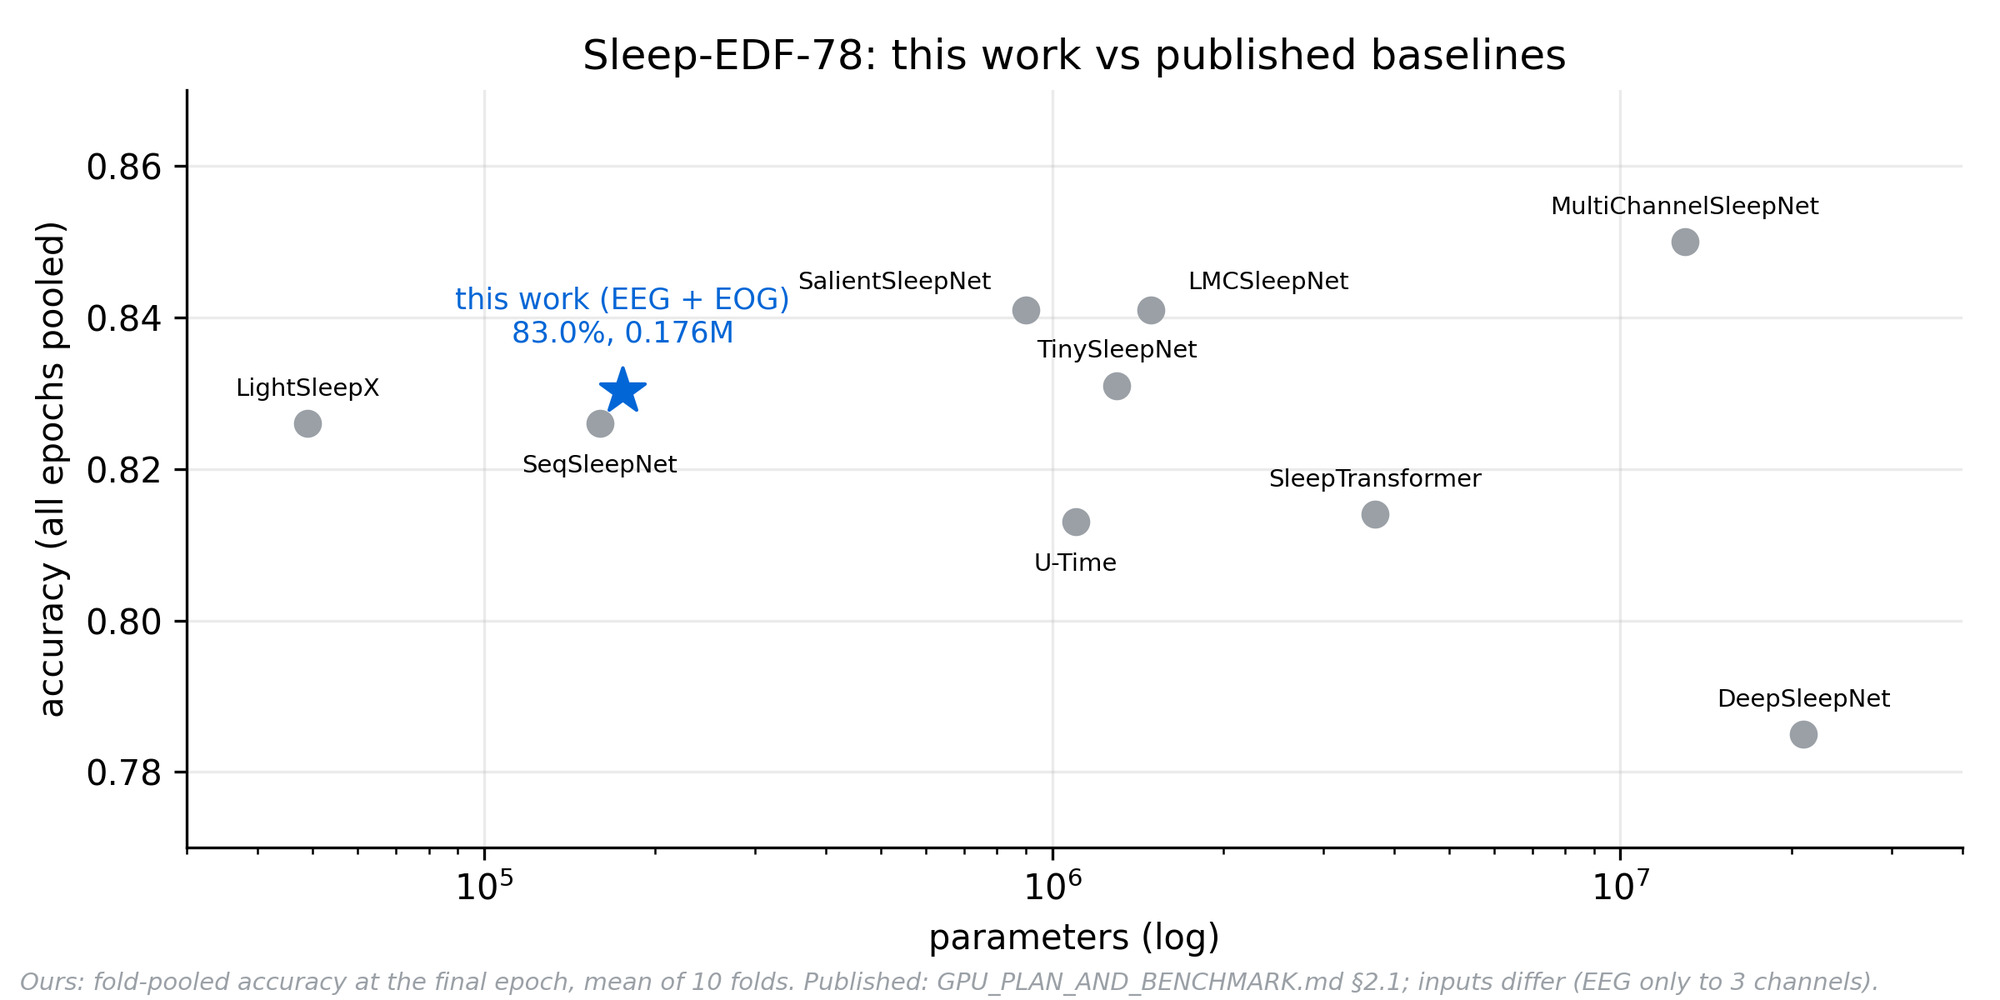
\includegraphics[width=0.85\textwidth]{F18_b1_vs_published.jpg}
\caption{B1 against published models on Sleep-EDF-78 (ours pooled like the papers, final epoch).}
\label{fig:b1pub}
\end{figure}

\begin{figure}[htbp]
\centering
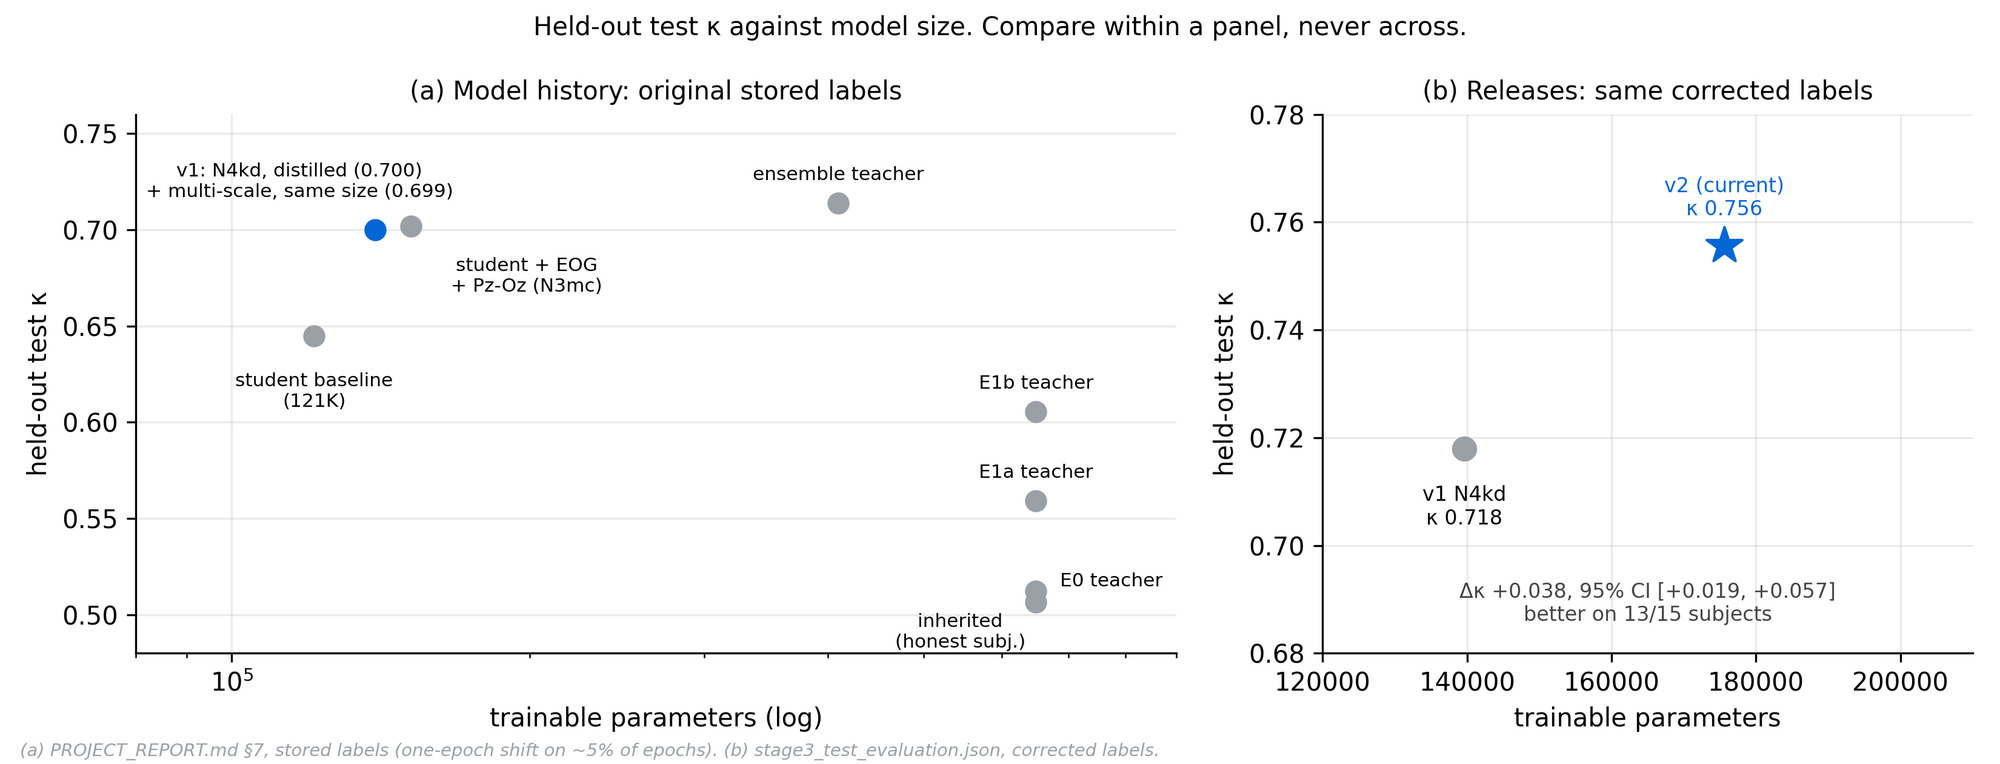
\includegraphics[width=0.85\textwidth]{F14_params_vs_kappa.jpg}
\caption{Model size against $\kappa$; v1 against v2 on the same corrected labels.}
\label{fig:size}
\end{figure}

\begin{figure}[htbp]
\centering
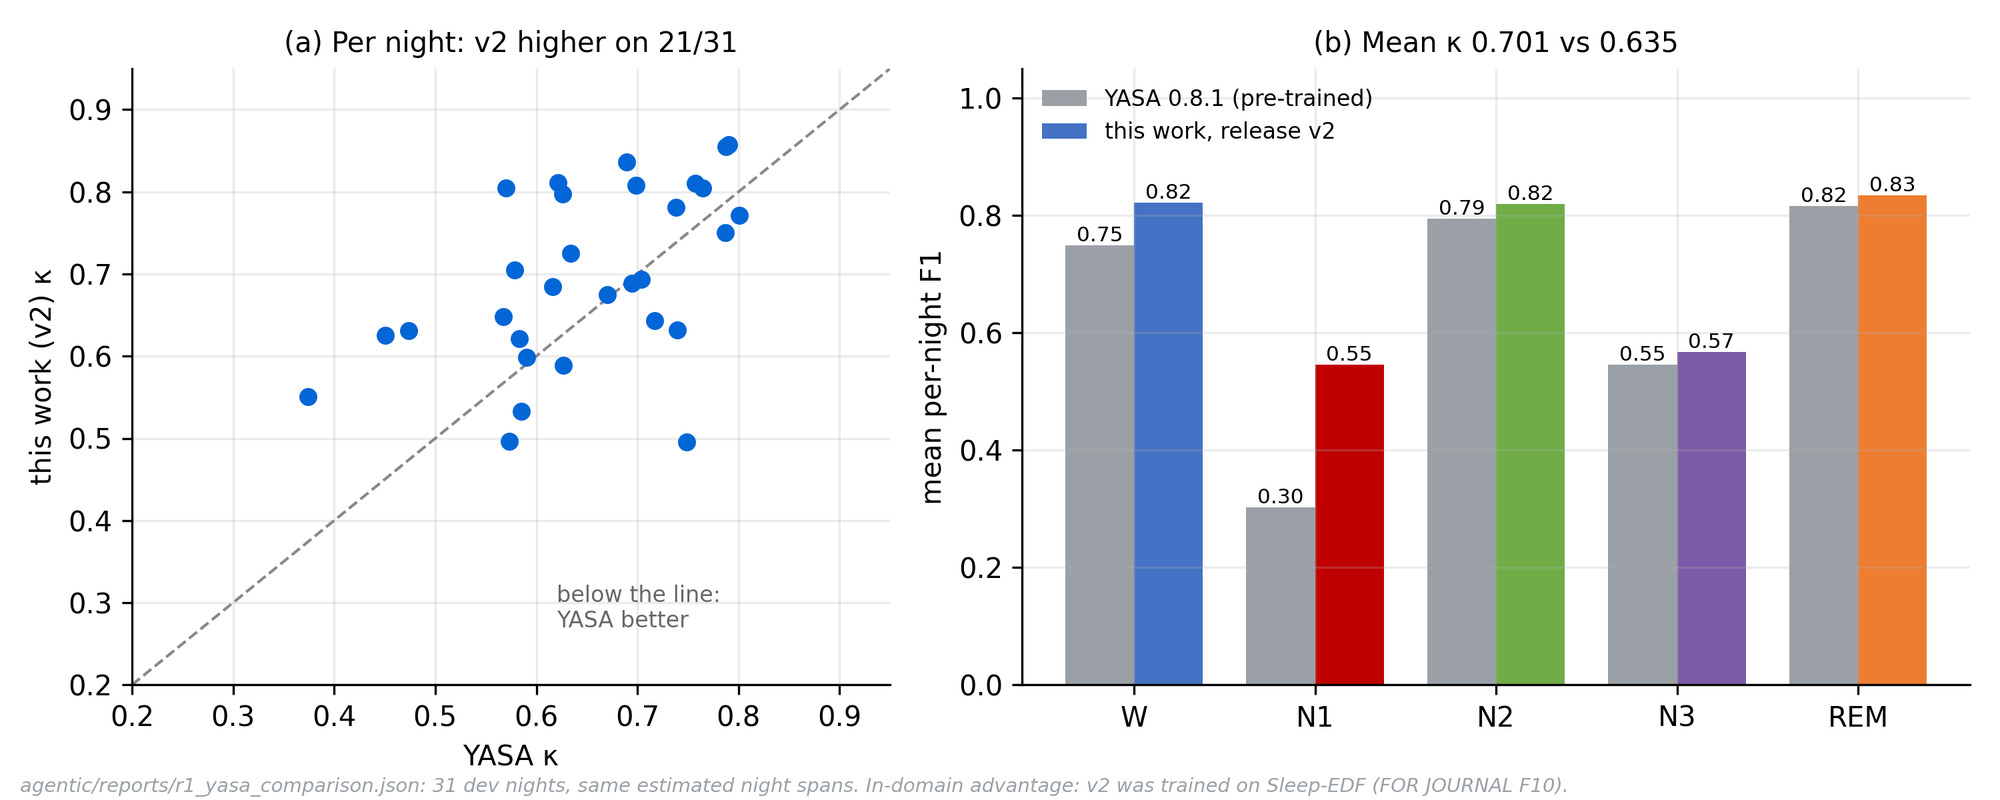
\includegraphics[width=0.85\textwidth]{F28_vs_yasa.jpg}
\caption{Same-night comparison with YASA on the 31 dev nights.}
\label{fig:yasa}
\end{figure}

\begin{table}[htbp]
\centering\small
\caption{Comparative analysis.}
\label{tab:compare}
\begin{tabularx}{\textwidth}{p{0.24\textwidth}Y}
\toprule
Comparison & Result \\
\midrule
Staging vs published (B1, Table~\ref{tab:published}) & $\kappa$ 0.769--0.775, level with TinySleepNet, LightSleepX and LMCSleepNet (0.77), below SleepSatelightFTC (0.787) and MultiChannelSleepNet (0.79); macro-F1 78.4--79.0 above TinySleepNet and LMCSleepNet; \textbf{175,599 parameters, 5--74$\times$ smaller} than the models at our level except LightSleepX (Figures~\ref{fig:b1pub}, \ref{fig:size}) \\
Per class (B1) & Strongest on N1 (51.6--53.1) and REM (85.7--85.9); weaker on N2 ($\sim$2 points below the best) and N3 ($\sim$3.5 points below) \\
Fair EEG-only comparison & \texttt{full\_eeg} CV $\kappa$ 0.765; test with EOG removed 0.744 \\
Same nights vs YASA 0.8.1 (31 dev nights) & Accuracy 0.790 vs 0.744; $\kappa$ 0.701 vs 0.635; macro-F1 0.717 vs 0.642; N1 F1 0.545 vs 0.302; better on 21/31 nights. Our model is in-domain; YASA is not (Figure~\ref{fig:yasa}) \\
vs our teacher & v2 beats ENSmc on every metric with 43\% of its parameters (combined effect of labels, EOG and recipe) \\
vs untrained SLM & Base Llama-3.2-3B: 2/31 at 5/5, and 31/31 flawed without the gate; v2 student: 31/31 dev, 28/29 test, 0 flawed released \\
vs LLM reporting systems (Table~\ref{tab:llm}) & Others check output after generation by humans or LLMs; ours blocks a report \textbf{before release} with a deterministic check, runs offline at temperature 0, and reruns byte-identically \\
Size & Staging model 0.70\,MB; the report model (2.02\,GB) is 99.9\% of the system footprint \\
\bottomrule
\end{tabularx}
\end{table}

\begin{table}[htbp]
\centering\scriptsize
\caption{Head-to-head scorecard against the best existing work. "Ours" figures are measured in this project (release v2 unless stated); verdicts are qualified where protocols differ.}
\label{tab:scorecard}
\begin{tabularx}{\textwidth}{p{0.17\textwidth}YYp{0.14\textwidth}}
\toprule
Aspect & Best existing (who, figure) & Ours & Verdict \\
\midrule
Automatic check of generated text & Human review or LLM-as-judge, after generation & Deterministic verifier before release; 0 flawed reports released on test (28/29 verified, 1 blocked) & \textbf{Ahead} \\
Complete report from a local model & Local LLMs on OSA: "needs significant improvement" (different task) & 31/31 dev and 28/29 test at 5/5; base model 2/31 & \textbf{Ahead} \\
Effect of the gate & No published ablation & Untrained model: 31/31 flawed without the gate, 0/31 with it & \textbf{Ahead} \\
Uncertainty in the report & Reported (SleepTransformer, YASA), not enforced in text & Hedging enforced by the verifier from measured error & \textbf{Ahead} \\
Offline and private & Local-LLM study (Seifen et al.) & Fully offline on CPU; network verified off in a container; 31/31 reports verified and identical there & \textbf{Ahead} \\
Reproducibility & Not reported & 31/31 byte-identical reruns; cross-platform staging parity 31/31 & \textbf{Ahead} \\
Student vs teacher & KD students usually approach the teacher & $\kappa$ 0.756 vs 0.732 on held-out test (confound disclosed) & \textbf{Ahead} (qualified) \\
Size for the accuracy & LightSleepX: 49\,K, $\kappa$ 0.77 & 176\,K, $\kappa$ 0.769--0.775 (B1) & Level \\
N1 F1 & SalientSleepNet 54.2 & 51.6--53.1 (B1) & Level \\
REM F1 & SalientSleepNet 85.8 & 85.7--85.9 (B1) & Level \\
Overall staging & MultiChannelSleepNet: 85.0\%, $\kappa$ 0.79, 13\,M & 83.0--83.5\%, $\kappa$ 0.769--0.775, 0.176\,M & Behind by $\sim$1.5 points, 74$\times$ smaller \\
N3 F1 & MultiChannelSleepNet 81.8 & 77.8--78.3 (B1) & Behind \\
External validation & SleepVLM (external cohort); SleepFM (SHHS) & None yet & Behind \\
Training data & SleepFM: $\sim$65,000 people & 85 subjects & Behind (by design) \\
Clinician evaluation & Seifen et al.; guidance-SLM human evaluation & None yet & Behind \\
Clinical scope & Products: apnea, arousals, leg movements & Staging and architecture only & Behind (out of scope) \\
Regulatory clearance & FDA 510(k), AASM certification & None & Behind (out of scope) \\
Edge hardware & Dreem 3S headband; Micro SleepNet on a phone & x86 container (4 CPUs / 16\,GB, offline) measured end to end; ARM64 staging parity in emulation; no Pi timing yet & Behind (planned) \\
\bottomrule
\end{tabularx}
\end{table}

\textbf{Summary: ahead on 7, level on 3, behind on 8.} The work leads on everything that makes a \emph{generated
report trustworthy}, matches the field on model size and the hard stages, and is behind on the evidence a clinic
would expect --- external validation, clinician rating, clinical scope and measured hardware --- which is exactly
the Phase~II plan in Chapter~5. The comparison with published staging models is indicative rather than exact:
their numbers are as published, on their own preprocessing and labels, whereas ours use corrected labels.
